\documentclass[12pt,a4paper]{article}
\usepackage{amsthm}
\usepackage{amsmath} 
\usepackage[serbian]{babel}

\usepackage{graphicx}
\usepackage{float}

\usepackage{multicol}

\newtheorem{thm}{Teorema}[section]
\theoremstyle{definition}
\newtheorem{dfn}{Definicija}[section]
\theoremstyle{remark}
\newtheorem{no}{Napomena}[section]
\theoremstyle{plain}
\newtheorem{lem}[thm]{Lema}

% text width and height
\textwidth 16cm
\textheight 23cm

% distance from the top
\voffset -1.5cm

% distance from the left
\hoffset 0cm
\oddsidemargin 0mm

% distance from the bottom
\footskip 1.5cm

\linespread{1}

\setlength\parindent{0pt}

\usepackage{minted}

\title{Primena fazi logike u obradi slika}
\author{Jelena Mrdak,\\ Tijana Jevti\' c}

\begin{document}
\maketitle

\begin{abstract}
  U ovom radu je predstavljena primena fazi logike u obradi slika. \\
  Njen zna\v caj za ovu oblast je pribli\v zen \v citaocu kroz detaljan opis nekoliko algoritama i uporedjivanjem rezultata istih sa nekim drugim nefazi metodama.\\ \\
  Da li metode za obradu slika zasnovane na fazi logici daju bolje rezultate od tradicionalnih metoda, da li su algoritmi slo\v zeniji, br\v zi ili pak,
  fazi logika nije uspela da nadje svoje mesto u ovoj oblasti, sazna\' cete \v citaju\' ci ovaj rad. \\ \\
  Kodovi su pisani u jeziku \textit{C++} pomo\' cu biblioteke \textit{OpenCV}. \\
  Napominjemo da su svi kodovi, kako oni navedeni u radu, tako i oni koji nisu, ali koji su kori\v s\' ceni za pore\dj enje, pisani ru\v cno od strane autora, te da svi rezultati i zaklju\v cci zavise od njihove implementacije. Tako\dj e prikazana vremena izvr\v savanja u velikoj meri zavise od ma\v sine na kojoj se kodovi izvr\v savaju, te mogu varirati, ali su sva vremena dobijena testiranjem na istom ra\v cunaru u sli\v cnim uslovima.
\end{abstract}

\newpage
\tableofcontents

\newpage
\section{Uvod}
U matematici smo do sad navikli da je ne\v sto ta\v cno ili neta\v cno, da ne\v sto pripada ili ne pripada skupu. Me\dj utim, nekad je te\v sko povu\' ci granicu i odrediti kad je ne\v sto 0, a kad 1. \v Sto smo bli\v zi granici, to nesigurnost ve\' ca. Na primer, ako \v zelimo da klasifikujemo ljude na niske i visoke i postavimo granicu na $170 cm$, dobijamo da je osoba visoka $170 cm$ visoka, dok je osoba visoka $169 cm$ niska, \v sto i nema mnogo smisla.\\

Fazi logiku je 1965. godine uveo Lotfi Zadeh i ona nam u velikoj meri mo\v ze pomo\' ci za re\v savanje pomenutih problema. \\
Peirce je bio jedan od prvih mislilaca koji se ozbiljnije pozabavio pitanjem neodredjenosti (eng. vagueness), jo\v s mnogo pre Zadeha., po\v cetkom 20. veka. 
Pierce nije verovao u jasnu razliku izmedju ta\v cnog i neta\v cnog, ve\' c u to da je \v zivot continuum.
Drugi poznati nau\v cnici i filozofi su se dalje bavili ovom idejom. Rasel je govorio: "Sav jezik je neodredjen. Neodredjenost je pitanje stepena (eng. Vagueness is a matter of degree)." [6]
\\ \\
Fazi skupovi se razlikuju od klasi\v cnih skupova kod kojih je granica jasna (element ili prripada ili ne pripada skupu). Zadeh je uop\v stio klasi\v cne skupove tako \v sto je pro\v sirio skup valuacije $\{0, 1\}$ na interval realnih brojeva $[0, 1]$. Stepen pripadnosti nekog elementa fazi skupu opisuje koliko taj element odgovara pojmu koji je reprezentovan fazi skupom. Konkretno, element $x$ pripada skupu $A$ sa stepenom $\mu_{A}(x)$, gde je $\mu_{A} : A \rightarrow [0, 1]$ karakteristi\v cna funkcija skupa $A$.\\

U ovom radu smo koristili upravo ove ideje kako bismo odredili da li je piksel crn ili beo, da li je piksel ivica ili nije, da li je dovoljno osvetljen ili ne.\\

Obrada slika kori\v s\' cenjem fazi logike nije jedinstvena teorija, ve\' c kolekcija razli\v citih fazi metoda za obradu slika, koji mogu da razumeju, opi\v su i 
obrade sliku, njene delove ili karakteristike, posmatraju\' ci je kao fazi skup. \\
Reprezentacija i obrada slike zavise od izabranog metoda i problema koji je potrebno re\v siti.
Najrazli\v citije fazi tehnike omogu\' cavaju odgovaraju\' ci okvir za napredak jer su zasnovane na znanju (eng. knowledge-based). [7] \\ 
Mogu da obrade podatke sa gre\v skom u sluc\v aju da je ista nastala usled neodredjenosti i dvosmislenosti (eng. ambiguity) (ali ne zbog nasumi\v cnosti (eng. randomness)). [4]
\\ \\ 
Fazi tehnike za obradu slika, uostalom kao i sve ostale fazi tehnike, sastoje se iz tri faze: fazifikacija, odgovaraju\' ca funkcija za promenu vrednosti funkcije pripadnosti 
i defazifikacija. Prva i poslednja faza su neophodne zbogtoga \v sto ne postoji odgovaraju\' ci fazi hardver. [7]
\\ \\ 
Slika $X$, koja se sastoji od M vrsta i N kolona, mo\v ze biti predstavljena kao
\begin{equation}
  X = \sum_{i=1}^{M}\sum_{j=1}^{N} x_{ij}, \mu_{ij}
\end{equation}
$\mu_{ij} \in [0, 1]$ i predstavlja vrednost funkcije pripadnosti.


\section{FCM}
\label{sec:FCM}
Fuzzy C-means (FCM) je jedan od najpopularnijih algoritama za fazi klasterovanje. U ovom poglavlju \' cemo ga najpre detaljno opisati, a zatim \' cemo ga iskoristiti za binarizaciju slike.\\

Cilj ovog algoritma je da skup $X=\{x_{1}, x_{2}, ..., x_{n}\}$ particioni\v se na $k$ delova (klastera) po 
nekom kriterijumu. Preciznije, kriterijum je minimizacija slede\' ce funkcije:
\begin{equation*}
 F(\bar{w}, \bar{c}) = \sum_{i=1}^{n}\sum_{j=1}^{k}w_{ij}^{m}\left\|x_{i}-c_{j}\right\|^{2},
\end{equation*}
gde $w_{ij}\in [0, 1]$ predstavlja pripadnost ta\v cke $x_{i}$ $j$-tom klasteru i $\sum_{j=1}^{k}w_{ij}=1$, dok je $c_{j}$ centroid $j$-tog klastera. Realni parametar $m>1$ predstavlja faktor fazifikacije i on se zadaje unapred.
U nastavku \' cemo preciznije odrediti ove koeficijente. Sada \' cemo samo ukratko opisati korake algoritma.\\

FCM je veoma sli\v can algoritmu k-means i sastoji se iz slede\' cih koraka:
\begin{itemize}
  \item Ako je slika u boji, konvertovati je u sivu. 
  \item Izabrati broj klastera $k$.
  \item Svakoj ta\v cki $x_{i}$ dodeliti koeficijente $w_{ij} \in [0, 1], j=1,2,..., k$.
  \item Ponavljati sve dok ne do\dj e do konvergencije:
    \begin{itemize}
      \item Izra\v cunati centroide za svaki klaster.
      \item A\v zurirati koeficijente.
    \end{itemize}
  \item Ta\v cku $x_{i}$ dodeliti klasteru kom najvi\v se pripada, tj. $r$-tom klasteru, gde je $w_{ir}=\max\limits_{j} w_{ij}$.
\end{itemize}

\begin{thm}
  Potrebni uslovi za minimizator $(\bar{w}^{*}, \bar{c}^{*})$ funkcije $F(\bar{w}, \bar{c})$ su:
  \begin{equation}\label{c}
    c_{j} = \frac{\sum\limits_{i=1}^{n} w_{ij}^m \cdot x_{i}}{\sum\limits_{i=1}^{n} w_{ij}^{m}}
  \end{equation}
  i
  \begin{equation}\label{w}
    w_{ij} = \frac{1}{\sum\limits_{u=1}^{k} \biggl(\frac{\left\|x_{i}-c_{j}\right\|}{\left\|x_{i}-c_{u}\right\|}\biggr)^{\frac{2}{m-1}}} 
  \end{equation}
\end{thm}
\begin{proof}
Prona\' ci \' cemo potencijalne ta\v cke lokalnih uslovnih ekstremuma. Koristi\' cemo Lagran\v zeve mno\v zioce. Posmatra\' cemo pomo\' cnu funkciju:
\begin{equation*}
  J(\bar{w}, \bar{c}, \bar{\lambda}) = \sum_{i=1}^{n}\sum_{j=1}^{k}w_{ij}^{m}\left\|x_{i}-c_{j}\right\|^{2} - \sum_{i=1}^{n}\lambda_{i}\biggl(\sum_{j=1}^{k}w_{ij}-1\biggr).
\end{equation*}

Ta\v cke koje tra\v zimo moraju da zadovoljavaju uslov $\nabla J=\textbf{0}$. Dakle,
  \begin{equation}\label{der_c}
  \frac{\partial J}{\partial c_{j}} = 0, 1\leq j \leq k
\end{equation}
  \begin{equation}\label{der_w}
  \frac{\partial J}{\partial w_{ij}} = 0, 1\leq i \leq n, 1\leq j \leq k 
\end{equation}
\begin{equation}\label{der_l}
  \frac{\partial J}{\partial \lambda_{i}} = 0, 1\leq i \leq n 
\end{equation}

  Re\v savanjem (\ref{der_c}) dobijamo (\ref{c}). Iz (\ref{der_w}) imamo
\begin{equation*}
  mw_{ij}^{m-1}\left\|x_{i}-c_{j}\right\|^{2} - \lambda_{i} = 0,
\end{equation*}
odnosno
\begin{equation}\label{wij}
  w_{ij} = \biggl(\frac{\lambda_{i}}{m\left\|x_{i}-c_{j}\right\|^{2}}\biggr)^{\frac{1}{m-1}}.
\end{equation}

Iz (\ref{der_l}) dobijamo:
\begin{align*}
  1&=\sum_{u=1}^{k}w_{iu}\\
   &=\sum_{u=1}^{k}\biggl(\frac{\lambda_{i}}{m\left\|x_{i}-c_{u}\right\|^{2}}\biggr)^{\frac{1}{m-1}}\\
   &=\sum_{u=1}^{k}\biggl(\frac{m\left\|x_{i}-c_{u}\right\|^{2}}{\lambda_{i}}\biggr)^{\frac{1}{1-m}}\\
   &=\sum_{u=1}^{k}\frac{(m\left\|x_{i}-c_{u}\right\|^{2})^{\frac{1}{1-m}}}{\lambda_{i}^{\frac{1}{1-m}}}\\
   &=\frac{1}{\lambda_{i}^{\frac{1}{1-m}}}\sum_{u=1}^{k}(m\left\|x_{i}-c_{u}\right\|^{2})^{\frac{1}{1-m}},
\end{align*}
pa zaklju\v cujemo da je
\begin{equation*}
  \lambda_{i} = \biggl(\sum_{u=1}^{k}(m\left\|x_{i}-c_{u}\right\|^{2})^{\frac{1}{1-m}}\biggr)^{1-m}.
\end{equation*}

Kona\v cno, zamenjuju\' ci poslednju jednakost u (\ref{wij}), dobijamo (\ref{w}). 
\end{proof}

FCM algoritam za odre\dj ivanje minimizatora funkcije $F$ je iteracija kroz potrebne uslove.

\subsection{Binarizacija slike}
\label{sec:binarizacija}
Ispod je prikazan kod za binarizaciju slike koji koristi FCM algoritam. Napominjemo da se zbog \v citljivosti koda u ovom delu nismo odlu\v cili za efikasnu implementaciju. O tome \' ce biti vi\v se re\v ci u narednoj sekciji.

\inputminted[tabsize=2,breaklines]{cpp}{codes/latex/binarization.cpp}

Rezultat izvr\v savanja algoritma je prikazan ispod.
\begin{multicols}{2}
% first column
\begin{figure}[H]
\centering
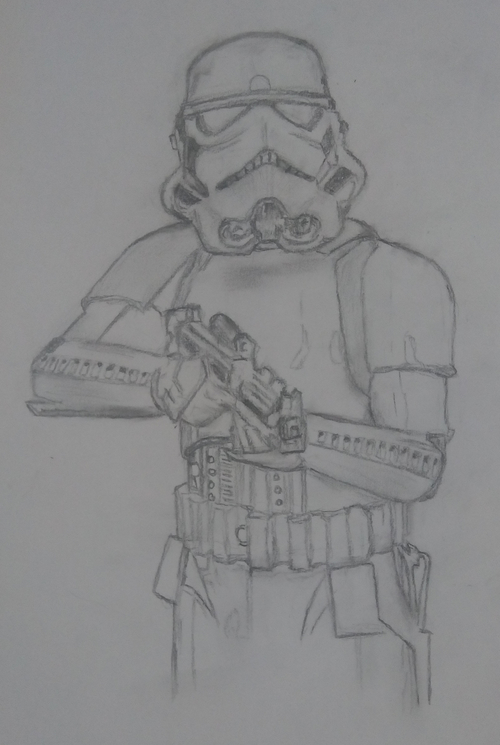
\includegraphics[width=5cm]{images/storm_trooper.jpg}
  \caption{input}\label{storm_trooper_input}
\end{figure}
\columnbreak
% second column
\begin{figure}[H]
\centering
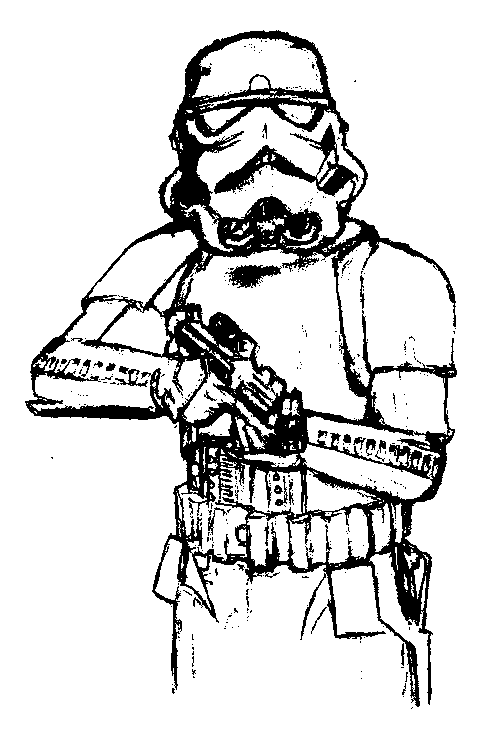
\includegraphics[width=5cm]{images/storm_trooper_binarized_fcm.png}
  \caption{output}
\end{figure}
\end{multicols}

\begin{multicols}{2}
% first column
\begin{figure}[H]
\centering
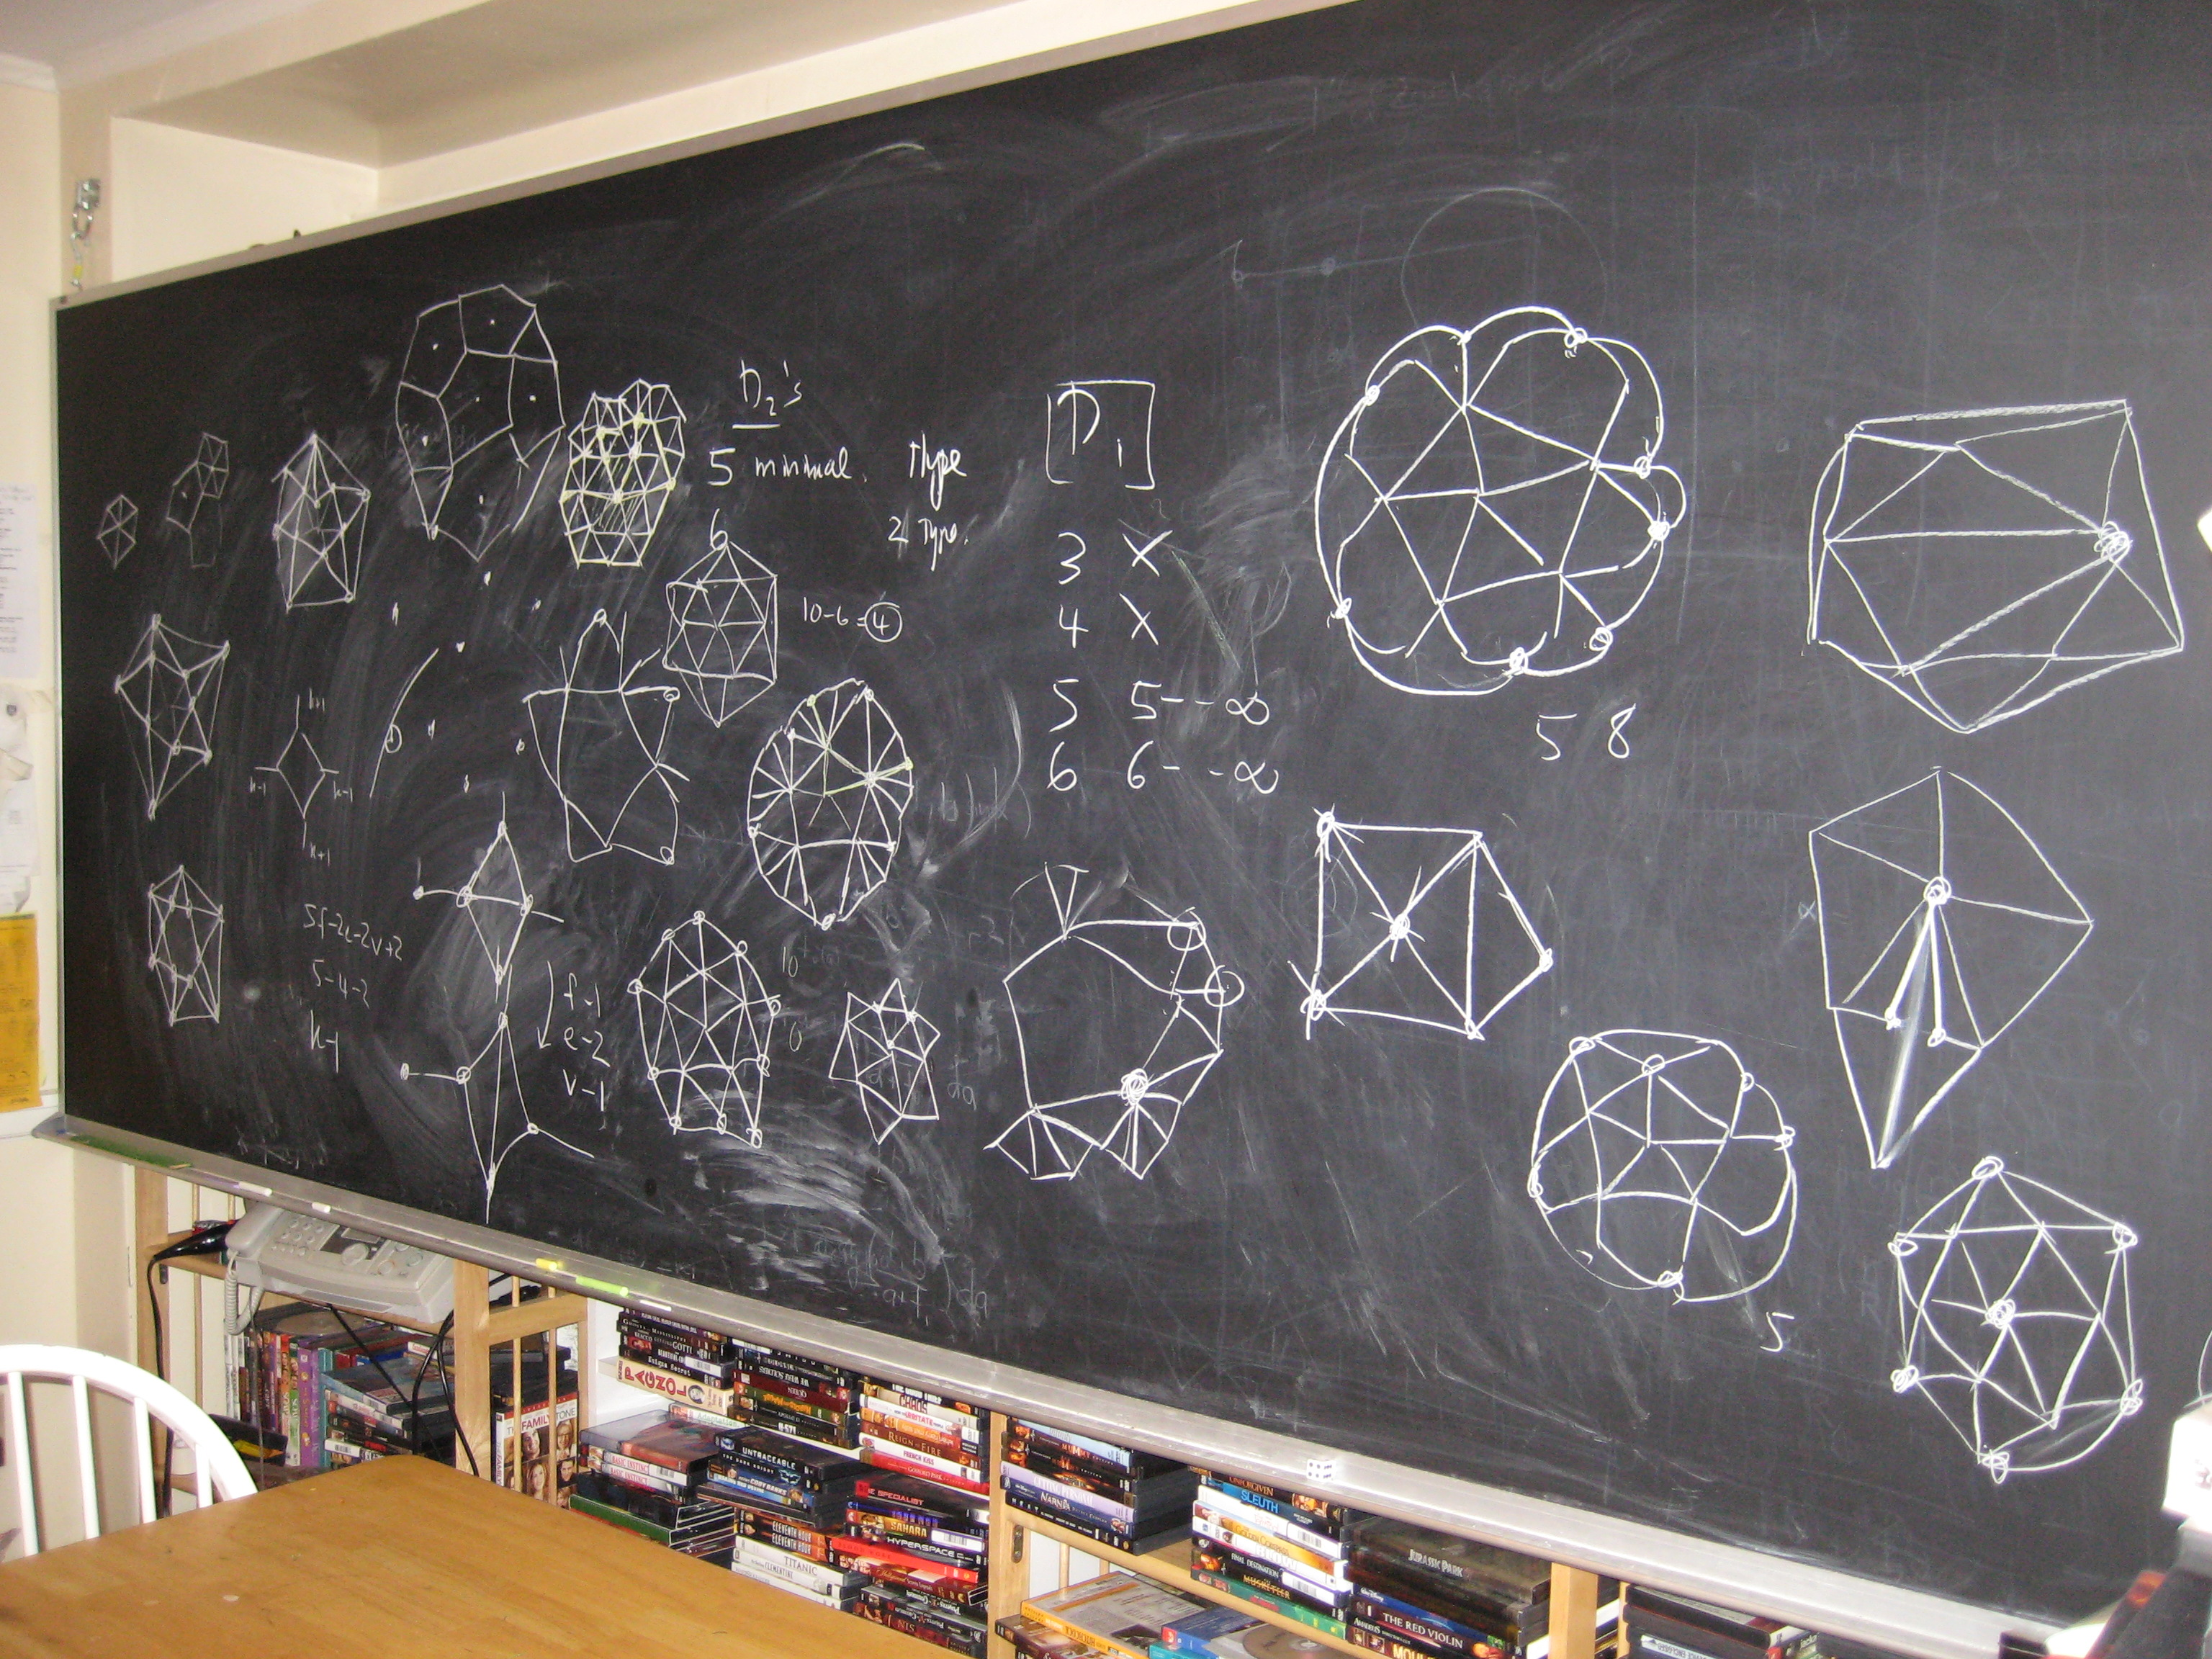
\includegraphics[width=7cm]{images/blackboard.jpg}
  \caption{input}\label{blackboard_input}
\end{figure}
\columnbreak
% second column
\begin{figure}[H]
\centering
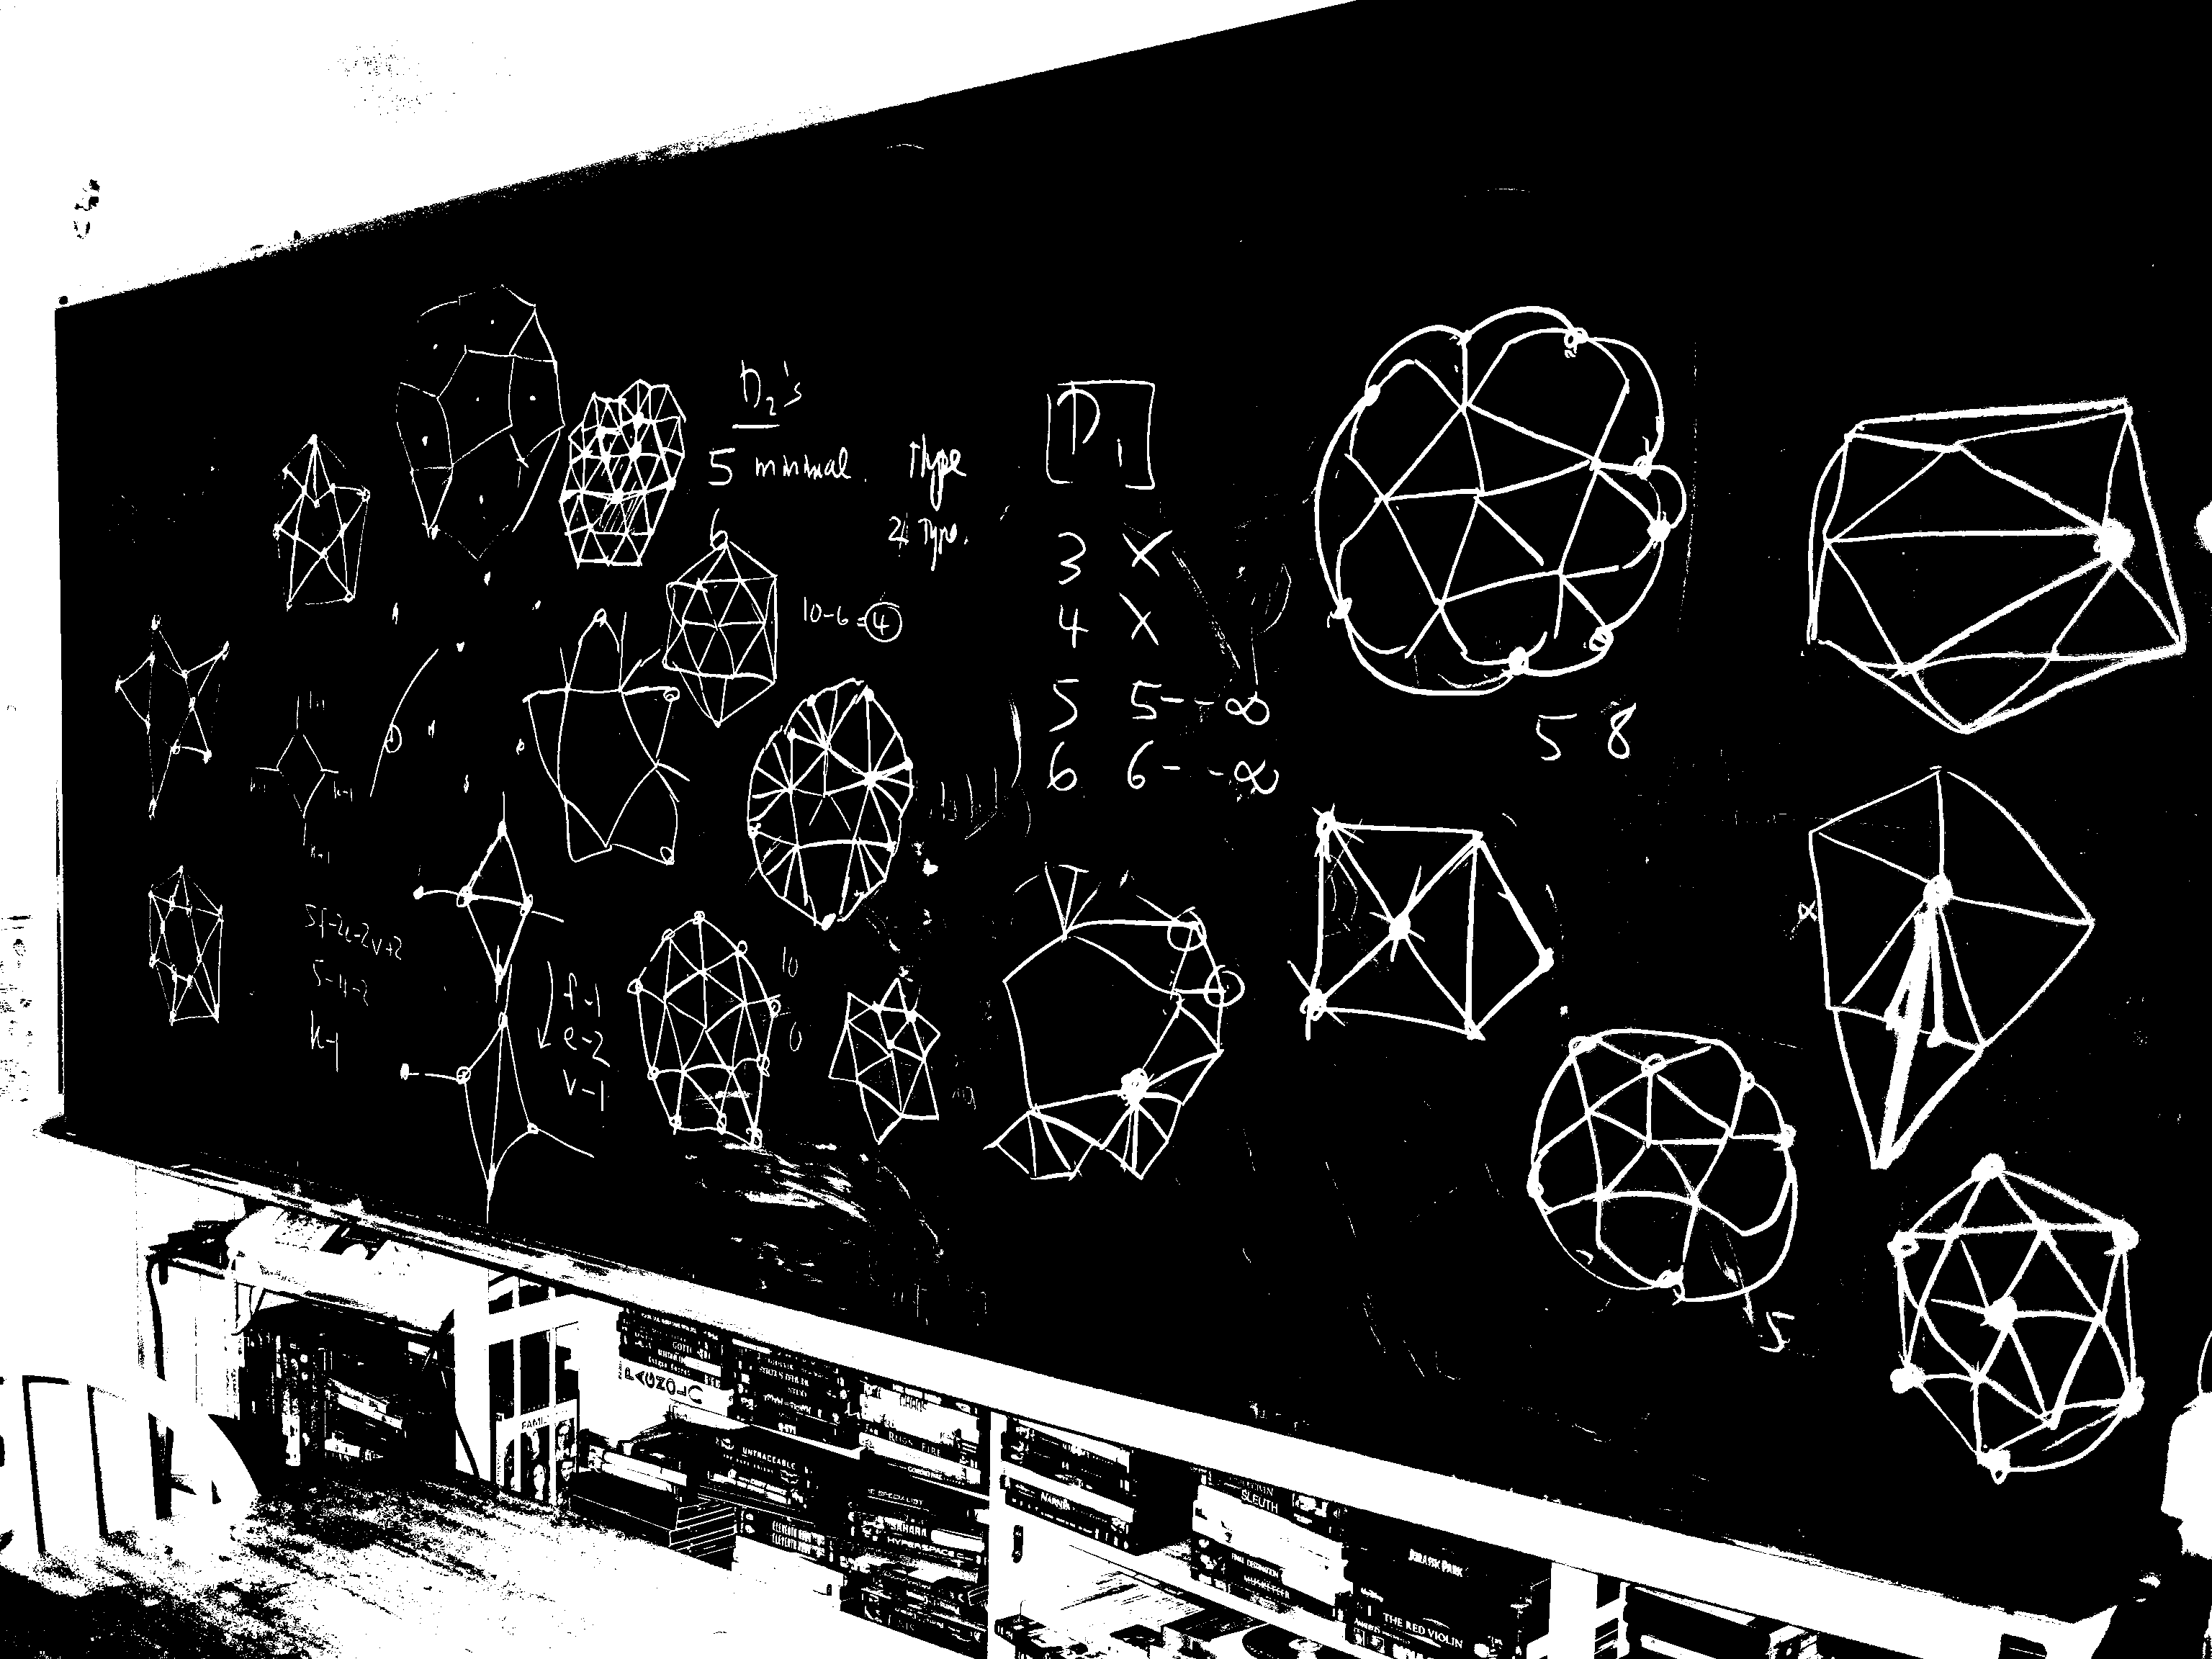
\includegraphics[width=7cm]{images/blackboard_binarized_fcm.png}
  \caption{output}
\end{figure}
\end{multicols}

\subsection{FCM i k-means}
U ovom odeljku \' cemo uporediti rezultate algoritama FCM i k-means, kao i vremena njihovih izvr\v savanja.

\begin{no}
  Koristi\' cemo efikasniju implementaciju FCM algoritma od one date u sekciji \ref{sec:binarizacija}.
\end{no}

Na slede\' cim slikama su prikazani rezultati.

\begin{multicols}{2}
% first column
\begin{figure}[H]
\centering
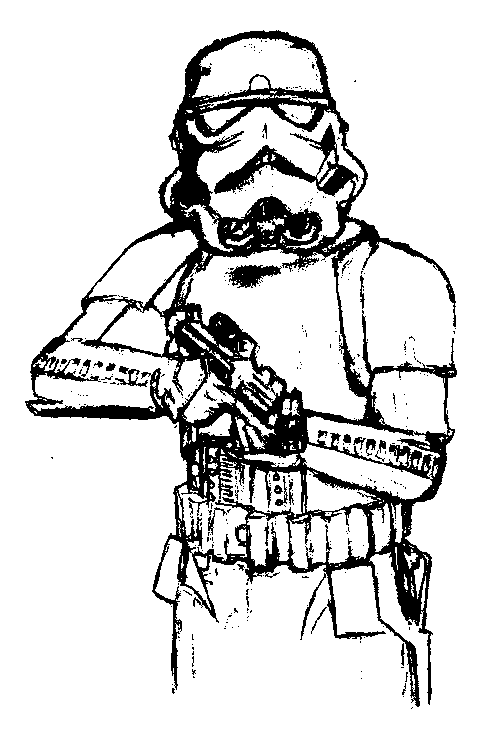
\includegraphics[width=5cm]{images/storm_trooper_binarized_fcm.png}
  \caption{FCM output}\label{storm_trooper_fcm}
 Broj iteracija: 7
\end{figure}
\columnbreak
% second column
\begin{figure}[H]
\centering
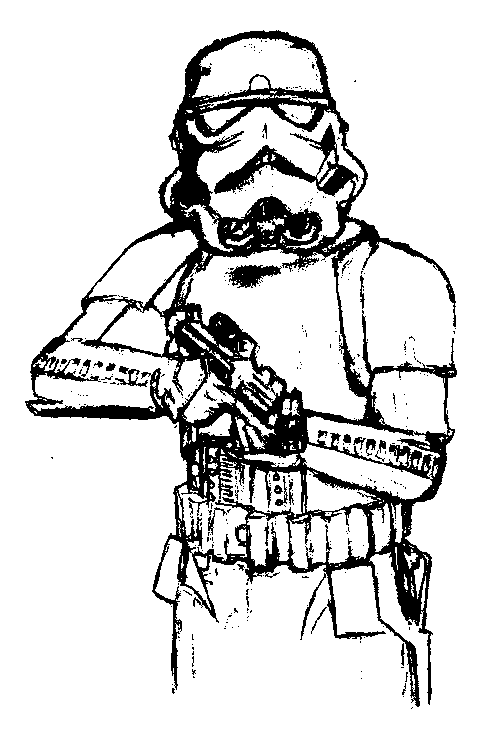
\includegraphics[width=5cm]{images/storm_trooper_binarized_kmeans.png}
  \caption{k-means output}\label{storm_trooper_kmeans}
 Broj iteracija: 6
\end{figure}
\end{multicols}

\newpage

\begin{multicols}{2}
% first column
\begin{figure}[H]
\centering
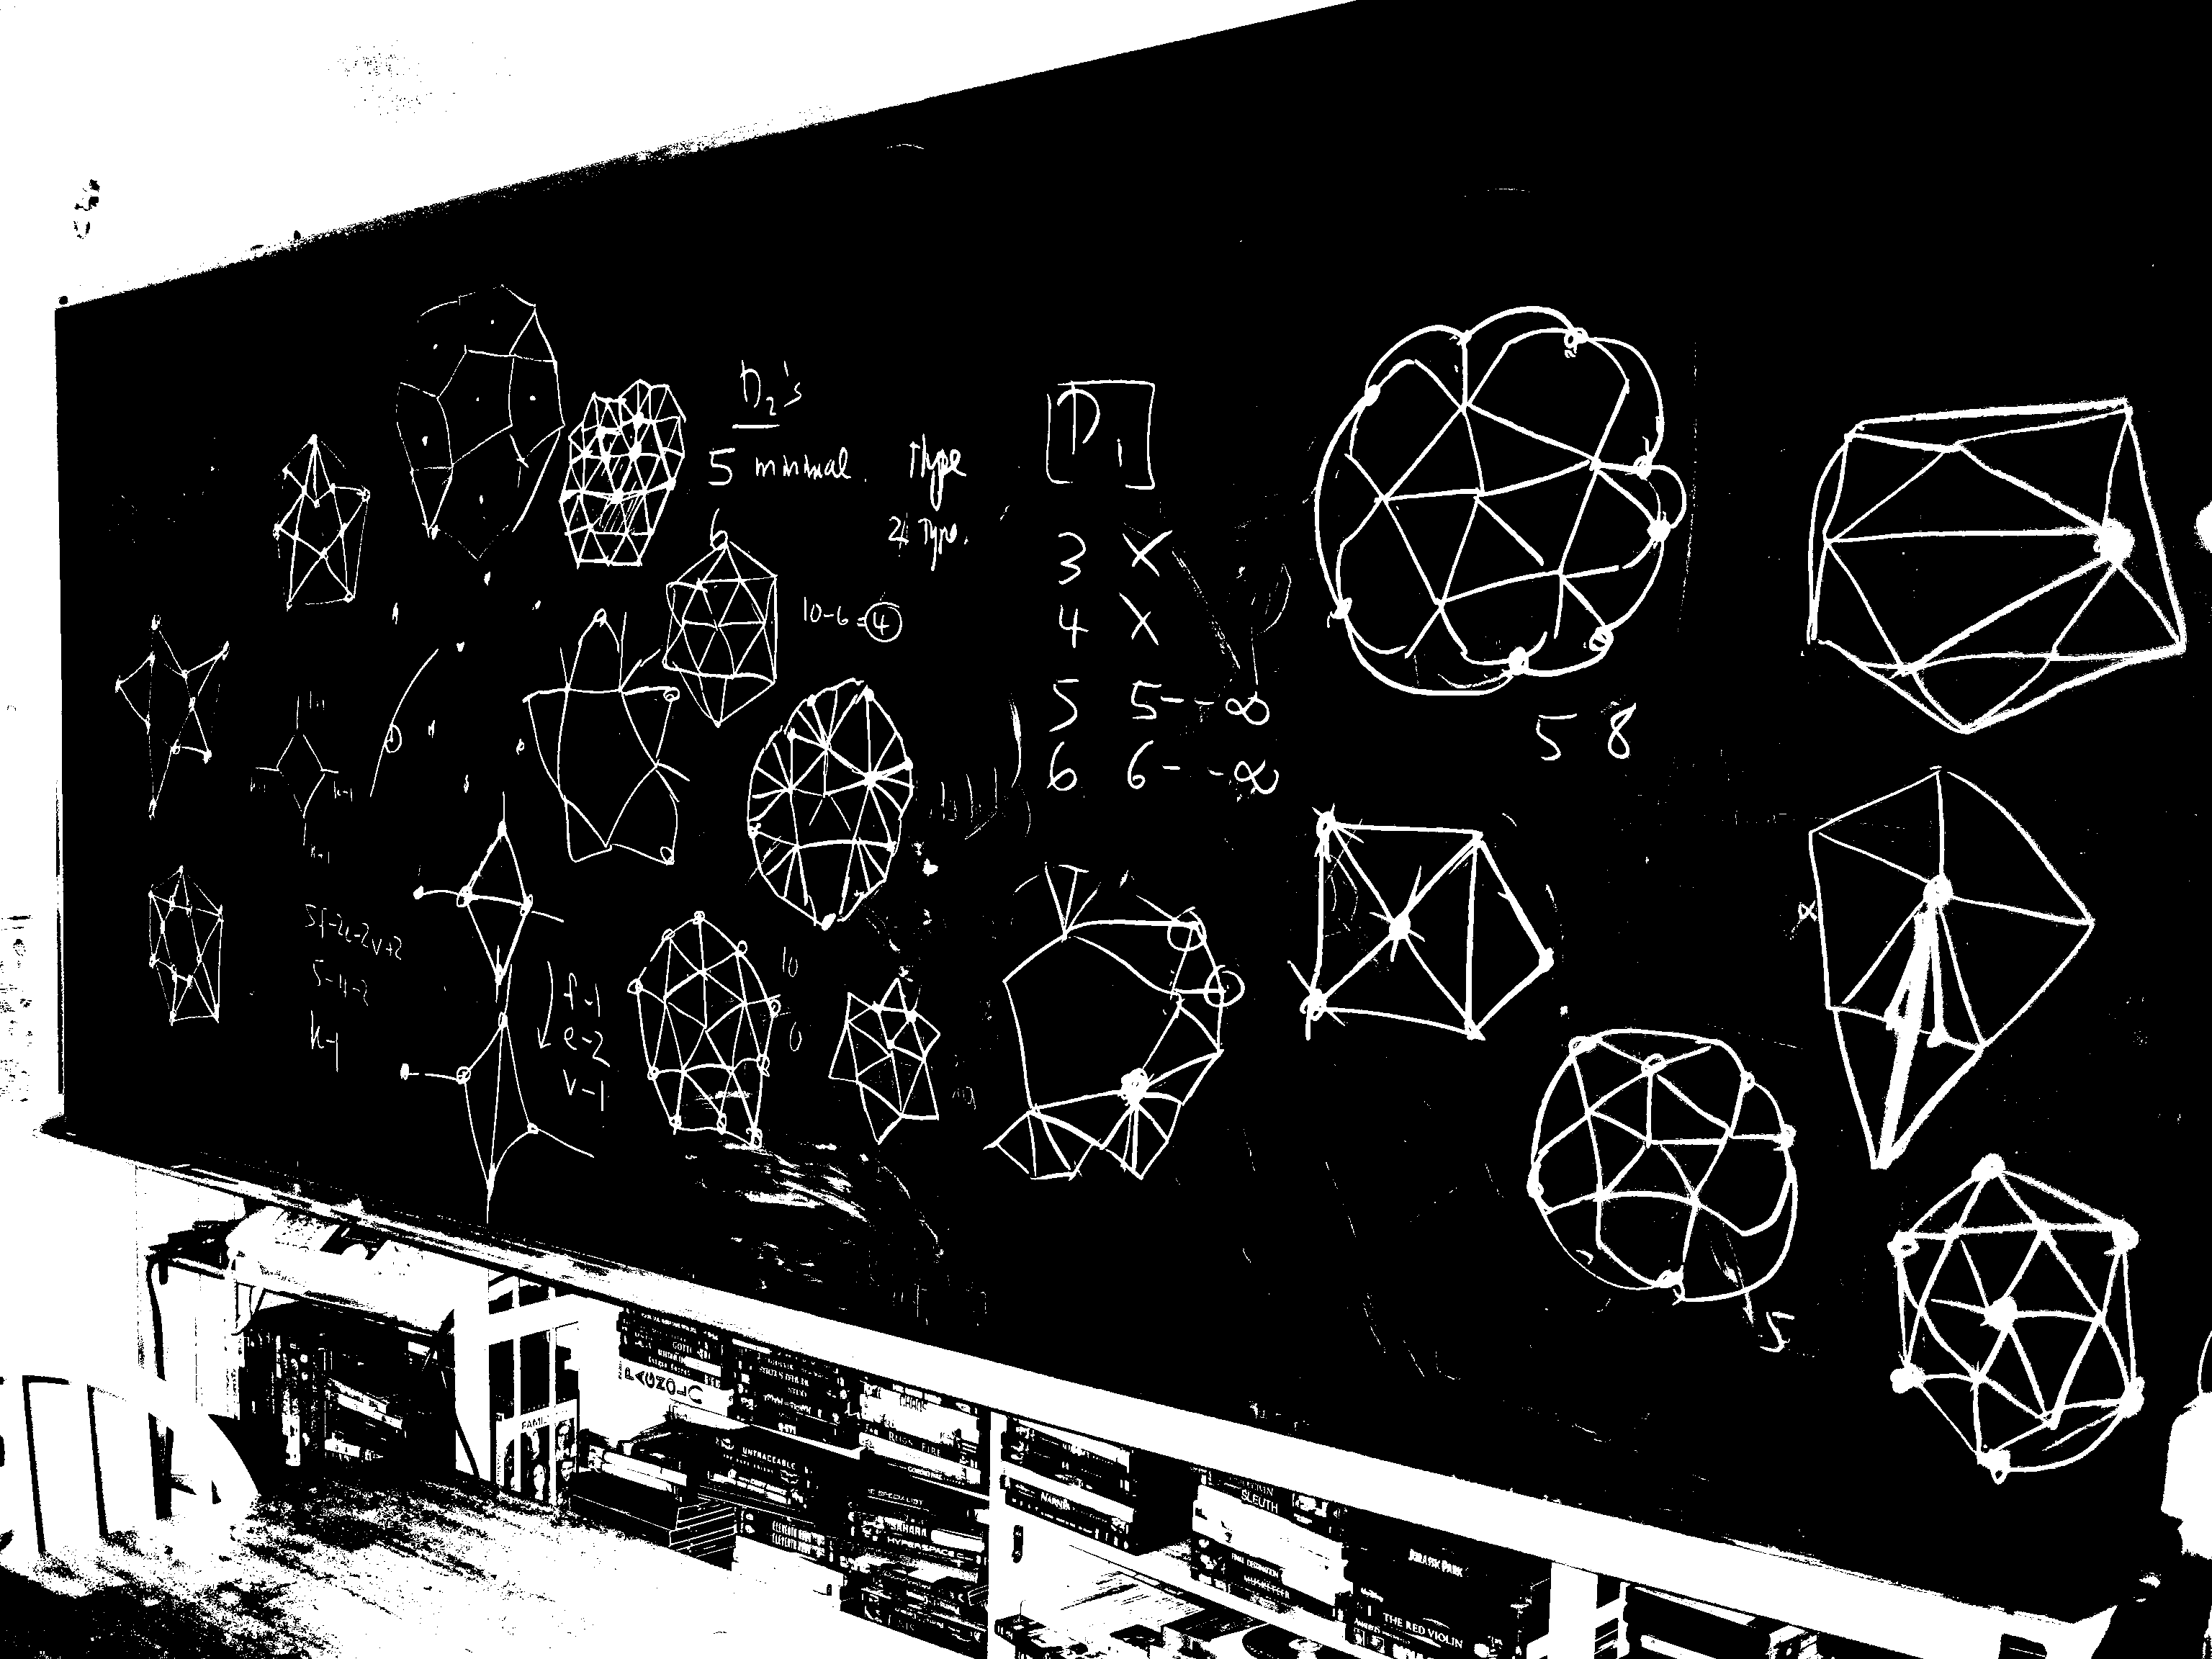
\includegraphics[width=7cm]{images/blackboard_binarized_fcm.png}
  \caption{FCM output}\label{blackboard_fcm}
 Broj iteracija: 7
\end{figure}
\columnbreak
% second column
\begin{figure}[H]
\centering
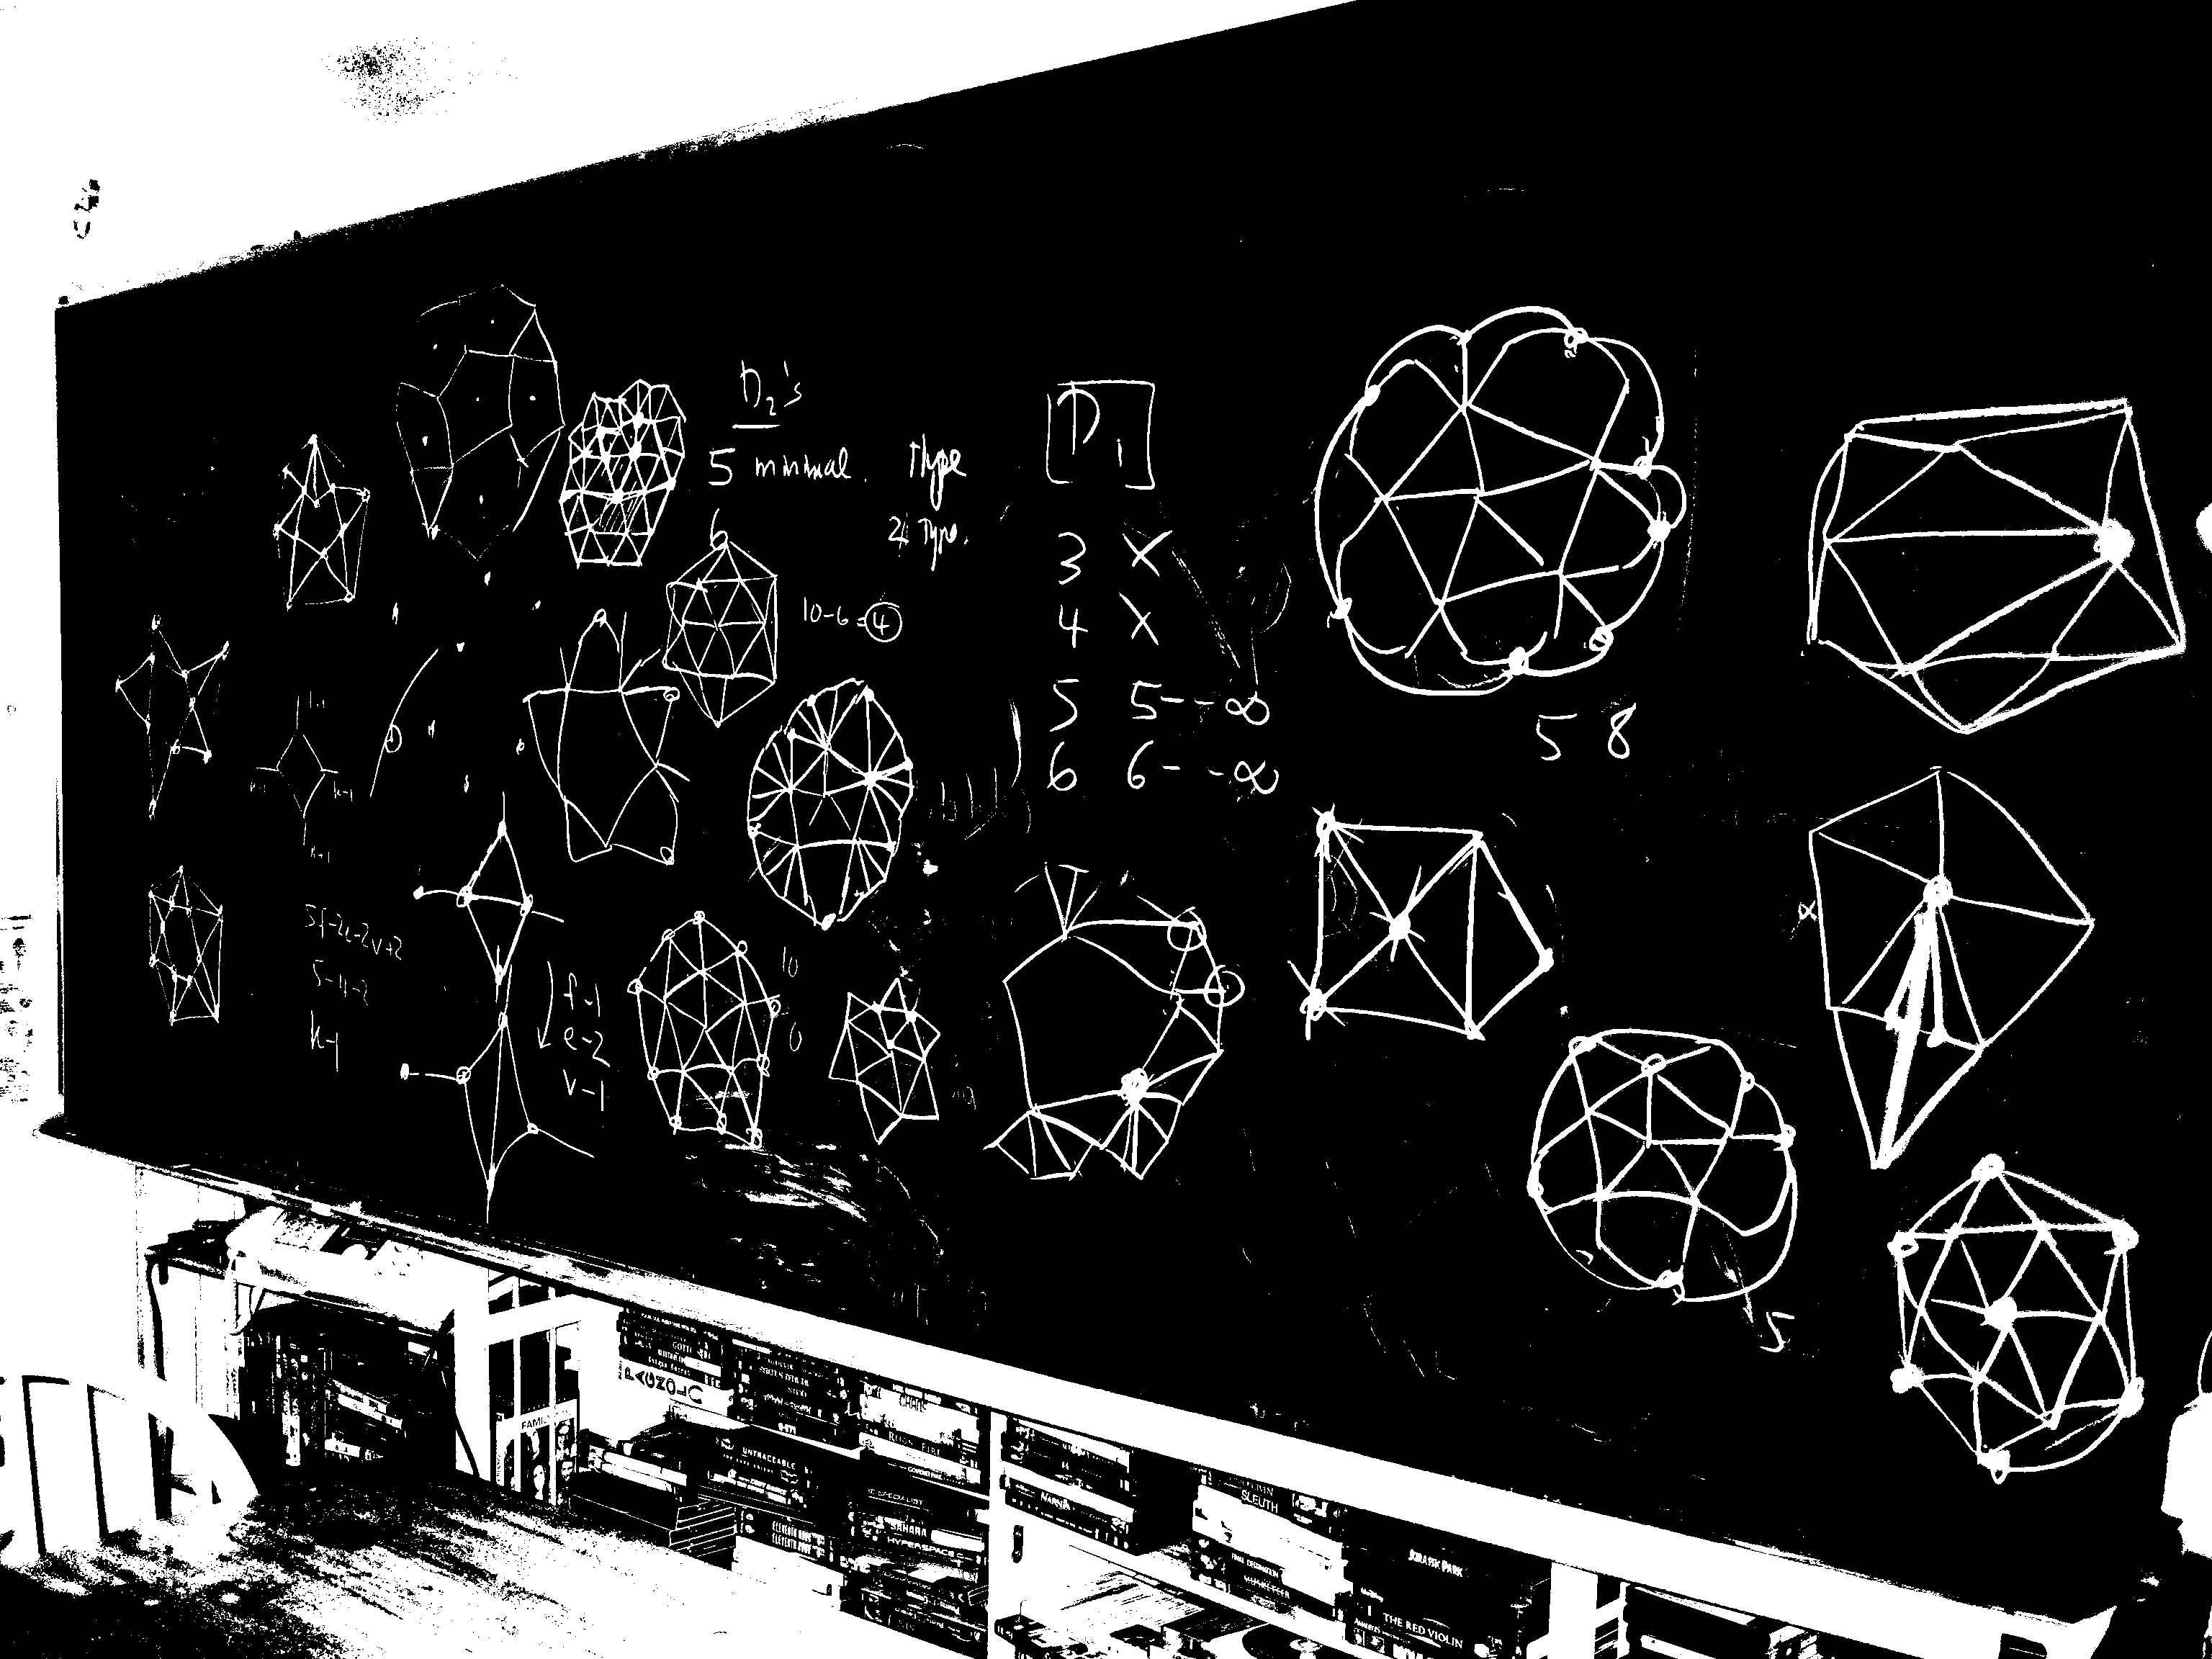
\includegraphics[width=7cm]{images/blackboard_binarized_kmeans.png}
  \caption{k-means output}\label{blackboard_kmeans}
  Broj iteracija: 7
\end{figure}
\end{multicols}

Mo\v zemo primetiti da su slike \ref{storm_trooper_fcm} i \ref{storm_trooper_kmeans} identi\v cne, dok se slike \ref{blackboard_fcm} i \ref{blackboard_kmeans} neznatno razlikuju. Me\dj utim, vremena izvr\v savanja se primetno razlikuju. U Tabeli \ref{vreme_storm} su prikazana vremena (u sekundama) potrebna da algoritmi obrade Sliku \ref{storm_trooper_input} 500, 1000 i 1500 puta. Sli\v cno, u Tabeli \ref{vreme_blackboard} su prikazana vremena potrebna da se obradi Slika \ref{blackboard_input} 50, 100 i 150 puta.

\begin{multicols}{2}
% first column
\begin{table}[H]
\centering
  \begin{tabular}{c|c|c}
  broj izvr\v savanja & FCM & k-means\\
  \hline
  500 & 4 & 21\\
  1000 & 8 & 42\\
  1500 & 12 & 63 
\end{tabular}
  \caption{Input Slika \ref{storm_trooper_input}}
  \label{vreme_storm}
\end{table}

\columnbreak

\begin{table}[H]
\centering
% second column
\begin{tabular}{c|c|c}
  broj izvr\v savanja & FCM & k-means\\
  \hline
  50 & 8 & 44\\
  100 & 17 & 89\\
  150 & 25 & 133 
\end{tabular}
  \caption{Input Slika \ref{blackboard_input}}
  \label{vreme_blackboard}
\end{table}
\end{multicols}

Prikaza\' cemo jo\v s dva testa ura\dj ena na dve nove slike.

\begin{multicols}{2}
% first column
\begin{table}[H]
\centering
  \begin{tabular}{c|c|c}
  broj izvr\v savanja & FCM & k-means\\
  \hline
    % mat
    100 & 15&  119 \\
    150&  22&  179 \\
    200&  31&  238
\end{tabular}
  \caption{}
\end{table}

\columnbreak

\begin{table}[H]
\centering
% second column
\begin{tabular}{c|c|c}
  broj izvr\v savanja & FCM & k-means\\
  \hline
% cat
  1000 & 3 & 36\\
  1500 & 5 & 53\\
  2000 & 6 & 71
\end{tabular}
  \caption{}
\end{table}
\end{multicols}

Na osnovu podataka iz tabela, zaklju\v cujemo:
\begin{table}[H]
\centering
\begin{tabular}{c|c}
  test & k-means/FCM\\
  \hline
  1 & 5 \\
  2 & 5 \\
  3 & 8 \\
  4 & 12
\end{tabular}
  \caption{Koliko puta je FCM br\v zi od k-means}
\end{table}

Treba napomenuti da su ovi rezultati okvirni, jer u velikoj meri zavise od implementacije samih algoritama. Naime, za centoride u k-means algoritmu je kori\v s\' cen celobrojni tip (int), dok je centroide u FCM algoritmu kori\v s\' cen realni tip (float). U oba slu\v caja su se algoritmi zaustavljali kad je promena u centroidima bila manja od jedan. Dakle, ve\' c tu mo\v ze do\' ci do razlike u broju iteracija. Me\dj utim, i dalje o\v cekujemo da \' ce FCM biti br\v zi od k-means.

Tako\dj e, isti\v cemo da FCM koristi vi\v se memorije nego k-means.

\section{Detekcija ivica}

Detekcija ivica ima veliki zna\v caj u obradi slika. Koristi se u raznim algoritmima kao \v sto su segmentacija slike, detekcija i izdvajanje karakteristika, pa \v cak nekad i u kompresiji slika.\\

Ivice mo\v zemo definisati kao mesta na slici gde se intenzitet naglo menja, tj. gde je razlika vrednosti susednih piksela velika. Postoje mnogi algoritmi koji se bave ovim problemom, me\dj utim, nijedan nije savr\v sen. Primerom \' cemo najbolje ilustrovati \v sta mislimo kad to ka\v zemo. Naime, Sobelov algoritam je dobar kada treba detektovati oblike, ali ne radi dobro u realnom vremenu gde je brzina klju\v cna (direktan prenos nekog doga\dj aja). Za takve situacije je prikladniji Canny algoritam.\\

U nastavku \' cemo videti jo\v s jedan pristup ovom problemu. Koristi\' cemo fazi logiku i fazi skupove.

\subsection{FED}

Kao \v sto smo ve\' c napomenuli, koristi\' cemo fazi logiku i fazi skupove da bismo detektovali ivice na slici. Preciznije, napravi\' cemo fazi skup koji sadr\v zi ure\dj ene parove (piksel, vrednost karakteristi\v cne funkcije). Taj skup \' ce predstavljati ivice, dok \' ce nam vrednosti karakteristi\v cne funkcije govoriti u kojoj meri piksel pripada tom skupu.

Postavlja se pitanje \v sta izabrati za karakteristi\v cnu funkciju. Podsetimo se, ivica je mesto gde se intenzitet naglo menja. Shodno tome, treba uzeti u obzir razliku intenziteta piksela koji trenutno posmatramo i njegovih suseda. Kada je ta razlika velika, vrednost na\v se funkcije treba da te\v zi jedinici, a kada je razlika mala, treba da te\v zi nuli. Jedna takva funkcija je:

\begin{equation}
  \mu_{edge}(p) = 1 - \frac{1}{1+\frac{\sum_{n\in N(p)}\left\|p-n\right\|}{L-1}},
\end{equation}

gde je $p$ piksel, $N(p)$ skup piksela iz njegove okoline, $L$ broj sivih nijansi (za 8-bitnu sliku, to je 256) i $\left\| \cdot \right\|$ norma koju \' cemo definisati kao apsolutnu vrednost razlike intenziteta piksela.\\

Pre nego \v sto damo kod, ukratko \' cemo opisati korake algoritma:
\begin{itemize}
  \item \textbf{Pretprocesiranje} - ako je slika u boji, konvertovati je u sivu sliku.
  \item \textbf{Pretprocesiranje} - primeniti Gausov filter na sliku kako bismo je malo zamutili.
  \item \textbf{Fazifikacija} - ra\v cunanje karakteristi\v cne funkcije $\mu_{edge}$ za svaki piksel sa slike. Takodje, \v cuvanje najve\' ce vrednosti funkcije (promenljiva MAX).
  \item \textbf{Normiranje vrednosti} - vrednosti karakteristi\v cne funkcije podeliti sa MAX:
    \begin{equation*}
      \mu_{edge}(p) = \frac{\mu_{edge}(p)}{MAX}
    \end{equation*}
  \item \textbf{Defazifikacija} - na osnovu vrednosti $\mu_{edge}(p)$ i nekog unapred datog praga (threshold), pikselu $p$ dodeliti crnu ili belu boju.
\end{itemize}

Po\v sto smo videli kratak opis algoritma, u nastavku dajemFCMo kod radi boljeg razumevanja istog.

\inputminted[tabsize=2,breaklines]{cpp}{codes/latex/edge_detection.cpp}

Na Slici \ref{fed_result} je prikazan rezultat rada algoritma.

\begin{multicols}{2}
% first column
\begin{figure}[H]
\centering
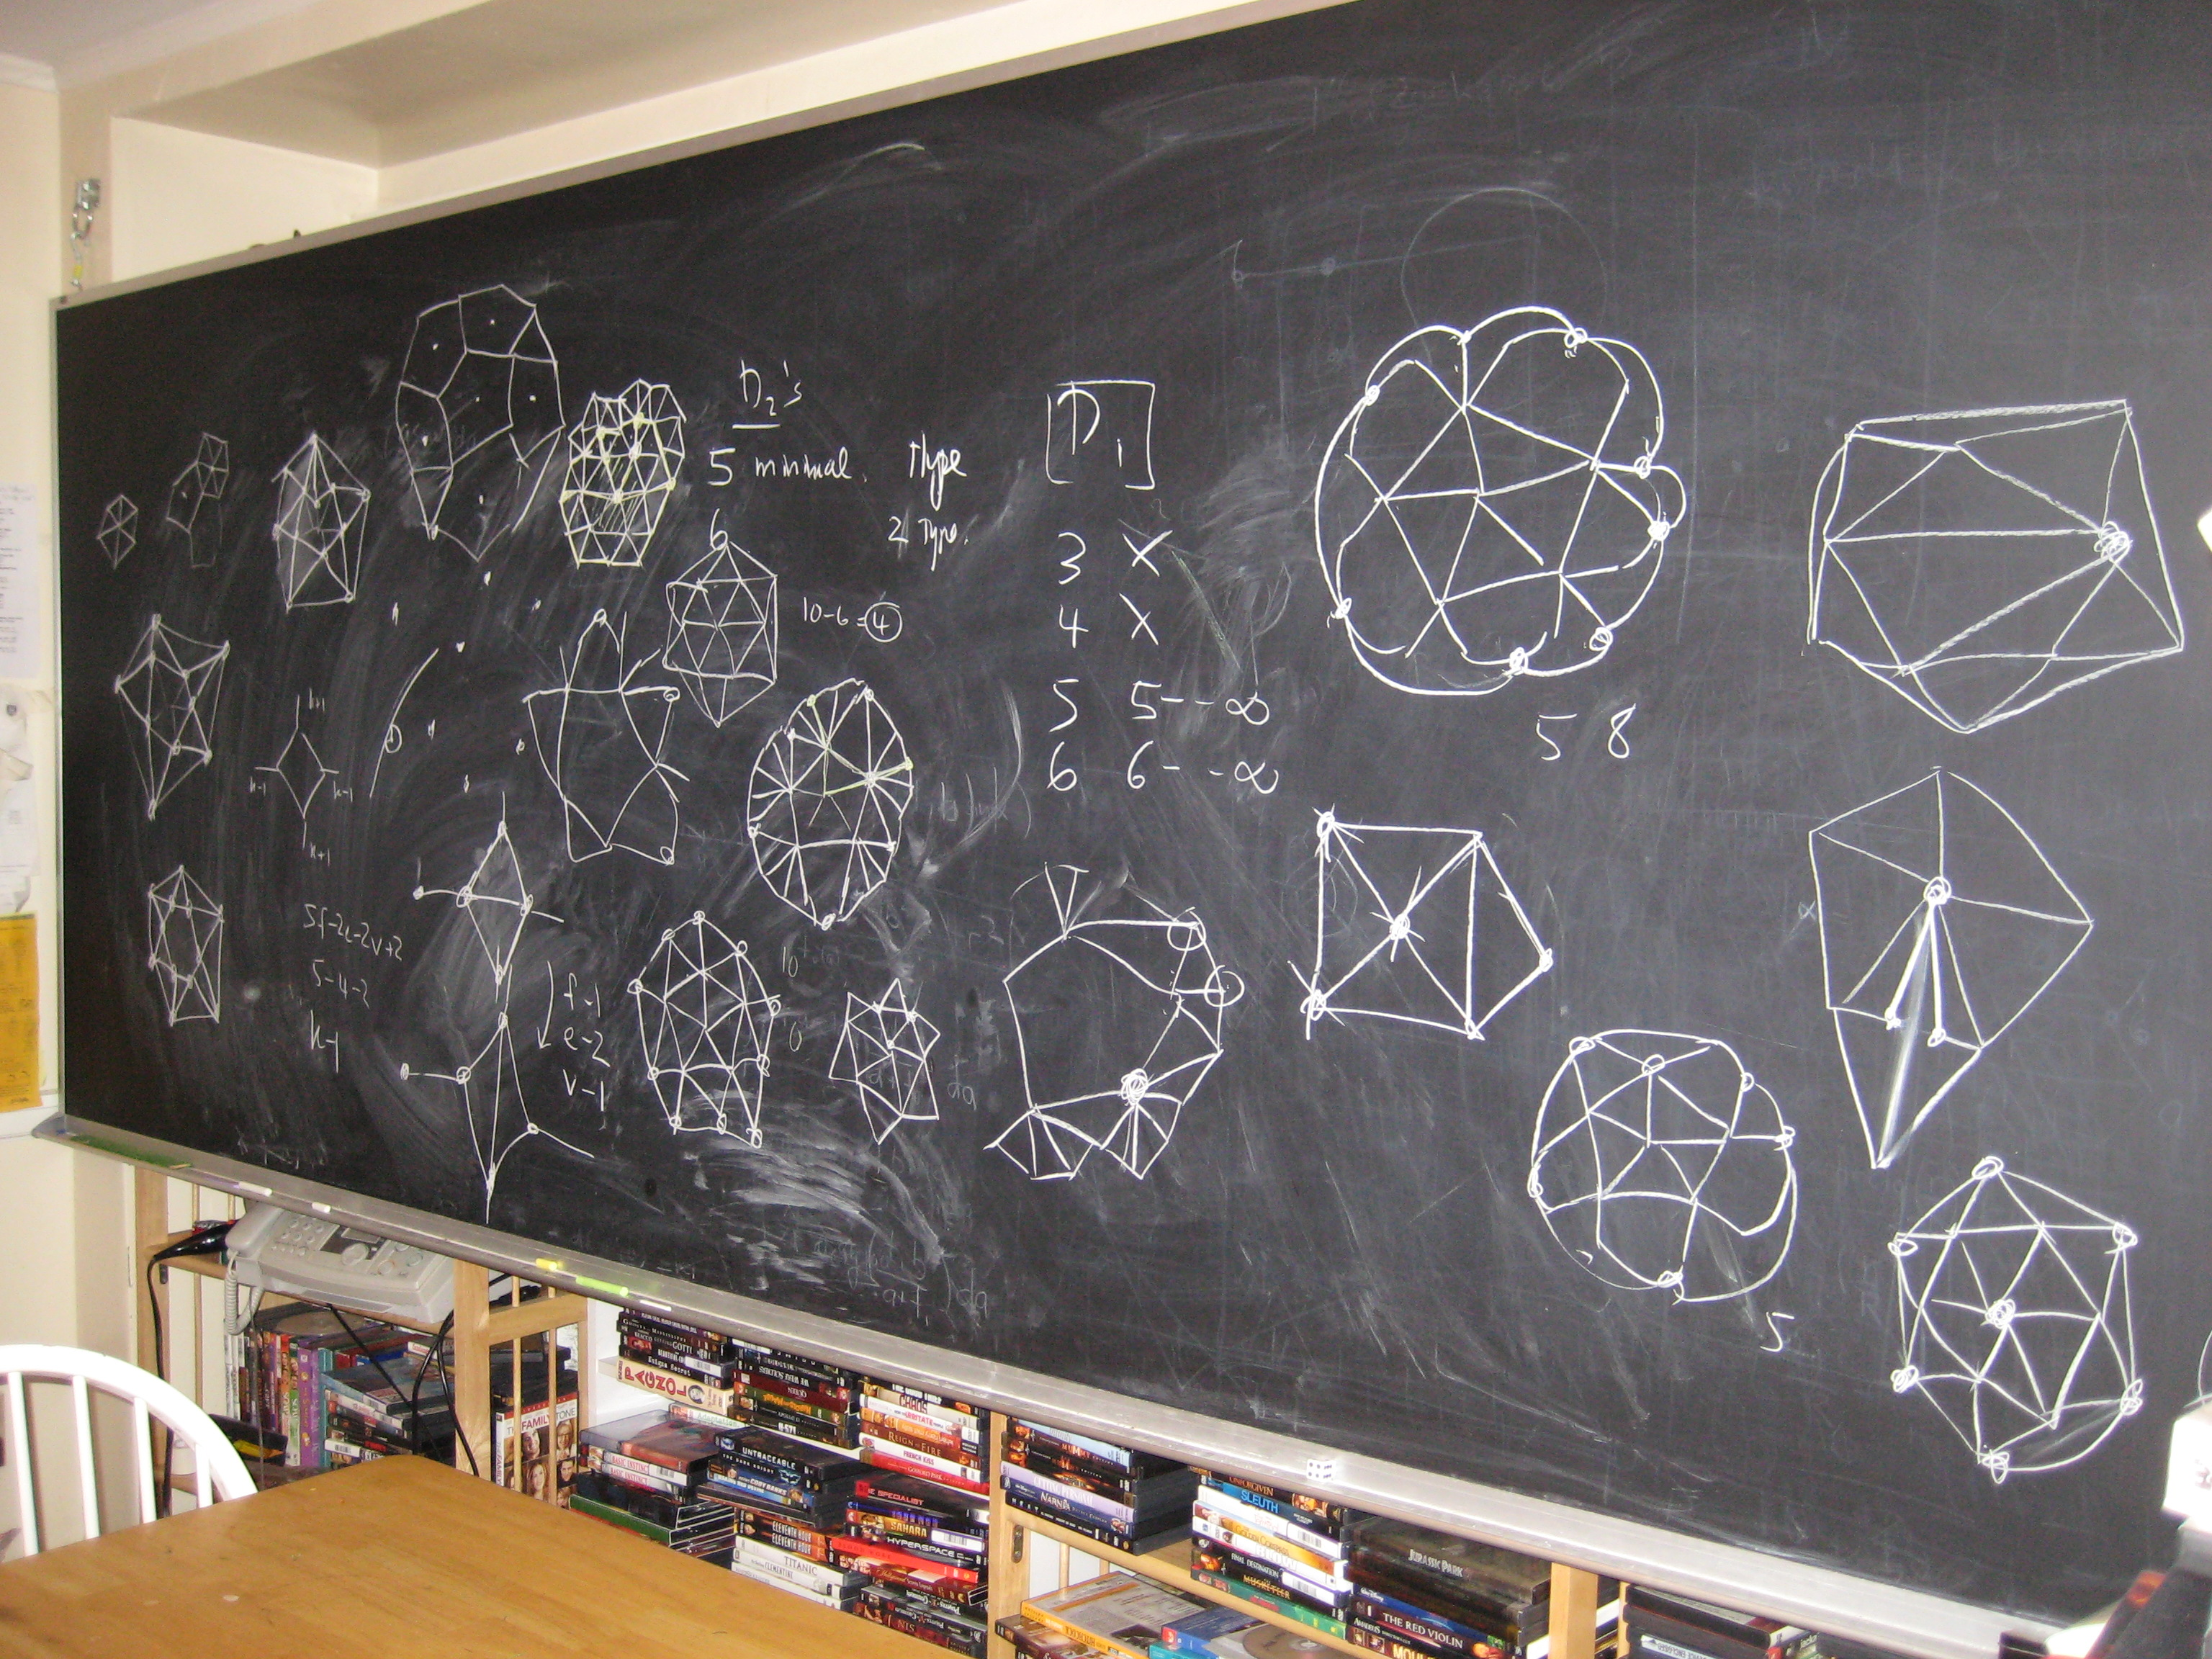
\includegraphics[width=7cm]{images/blackboard.jpg}
  \caption{input}\label{blackboard_fed_input}
\end{figure}
\columnbreak
% second column
\begin{figure}[H]
\centering
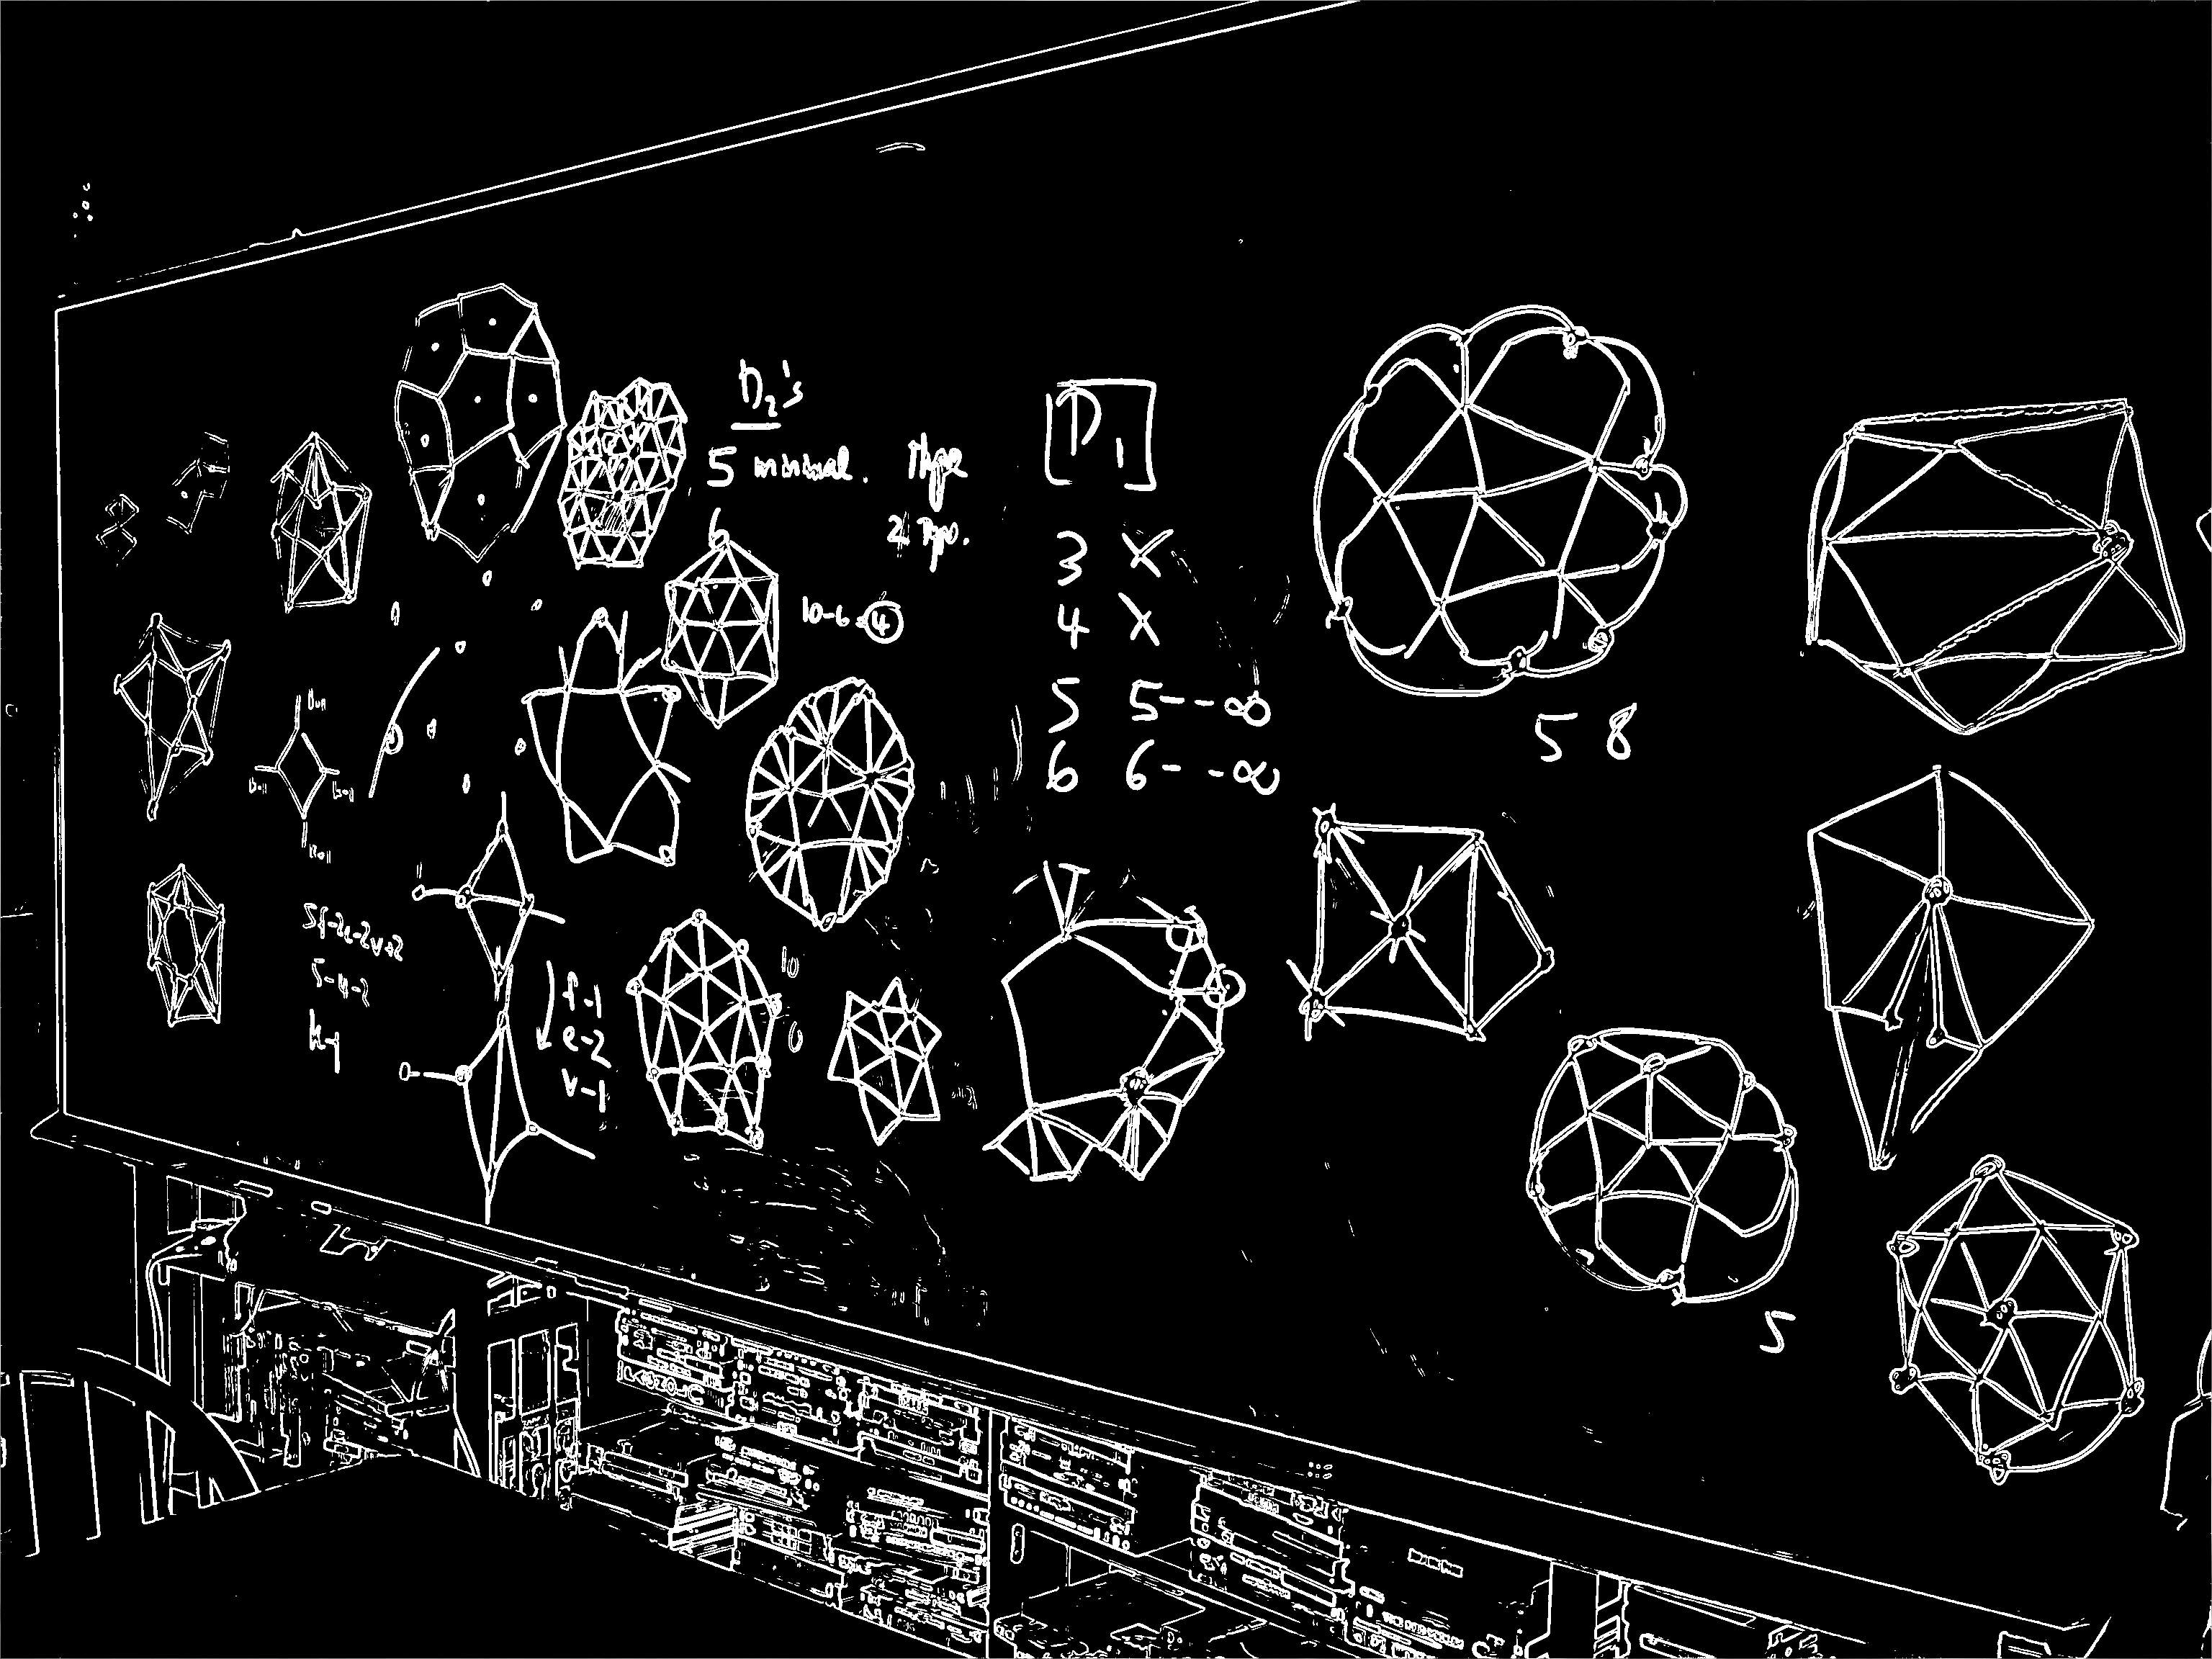
\includegraphics[width=7cm]{images/blackboard_35.png}
  \caption{output}\label{fed_result}
\end{figure}
\end{multicols}

Na slede\' cim slikama mo\v zemo videti kako se rezultat menja u zavisnosti od praga koji se zadaje.

\begin{multicols}{3}
% first column
\begin{figure}[H]
\centering
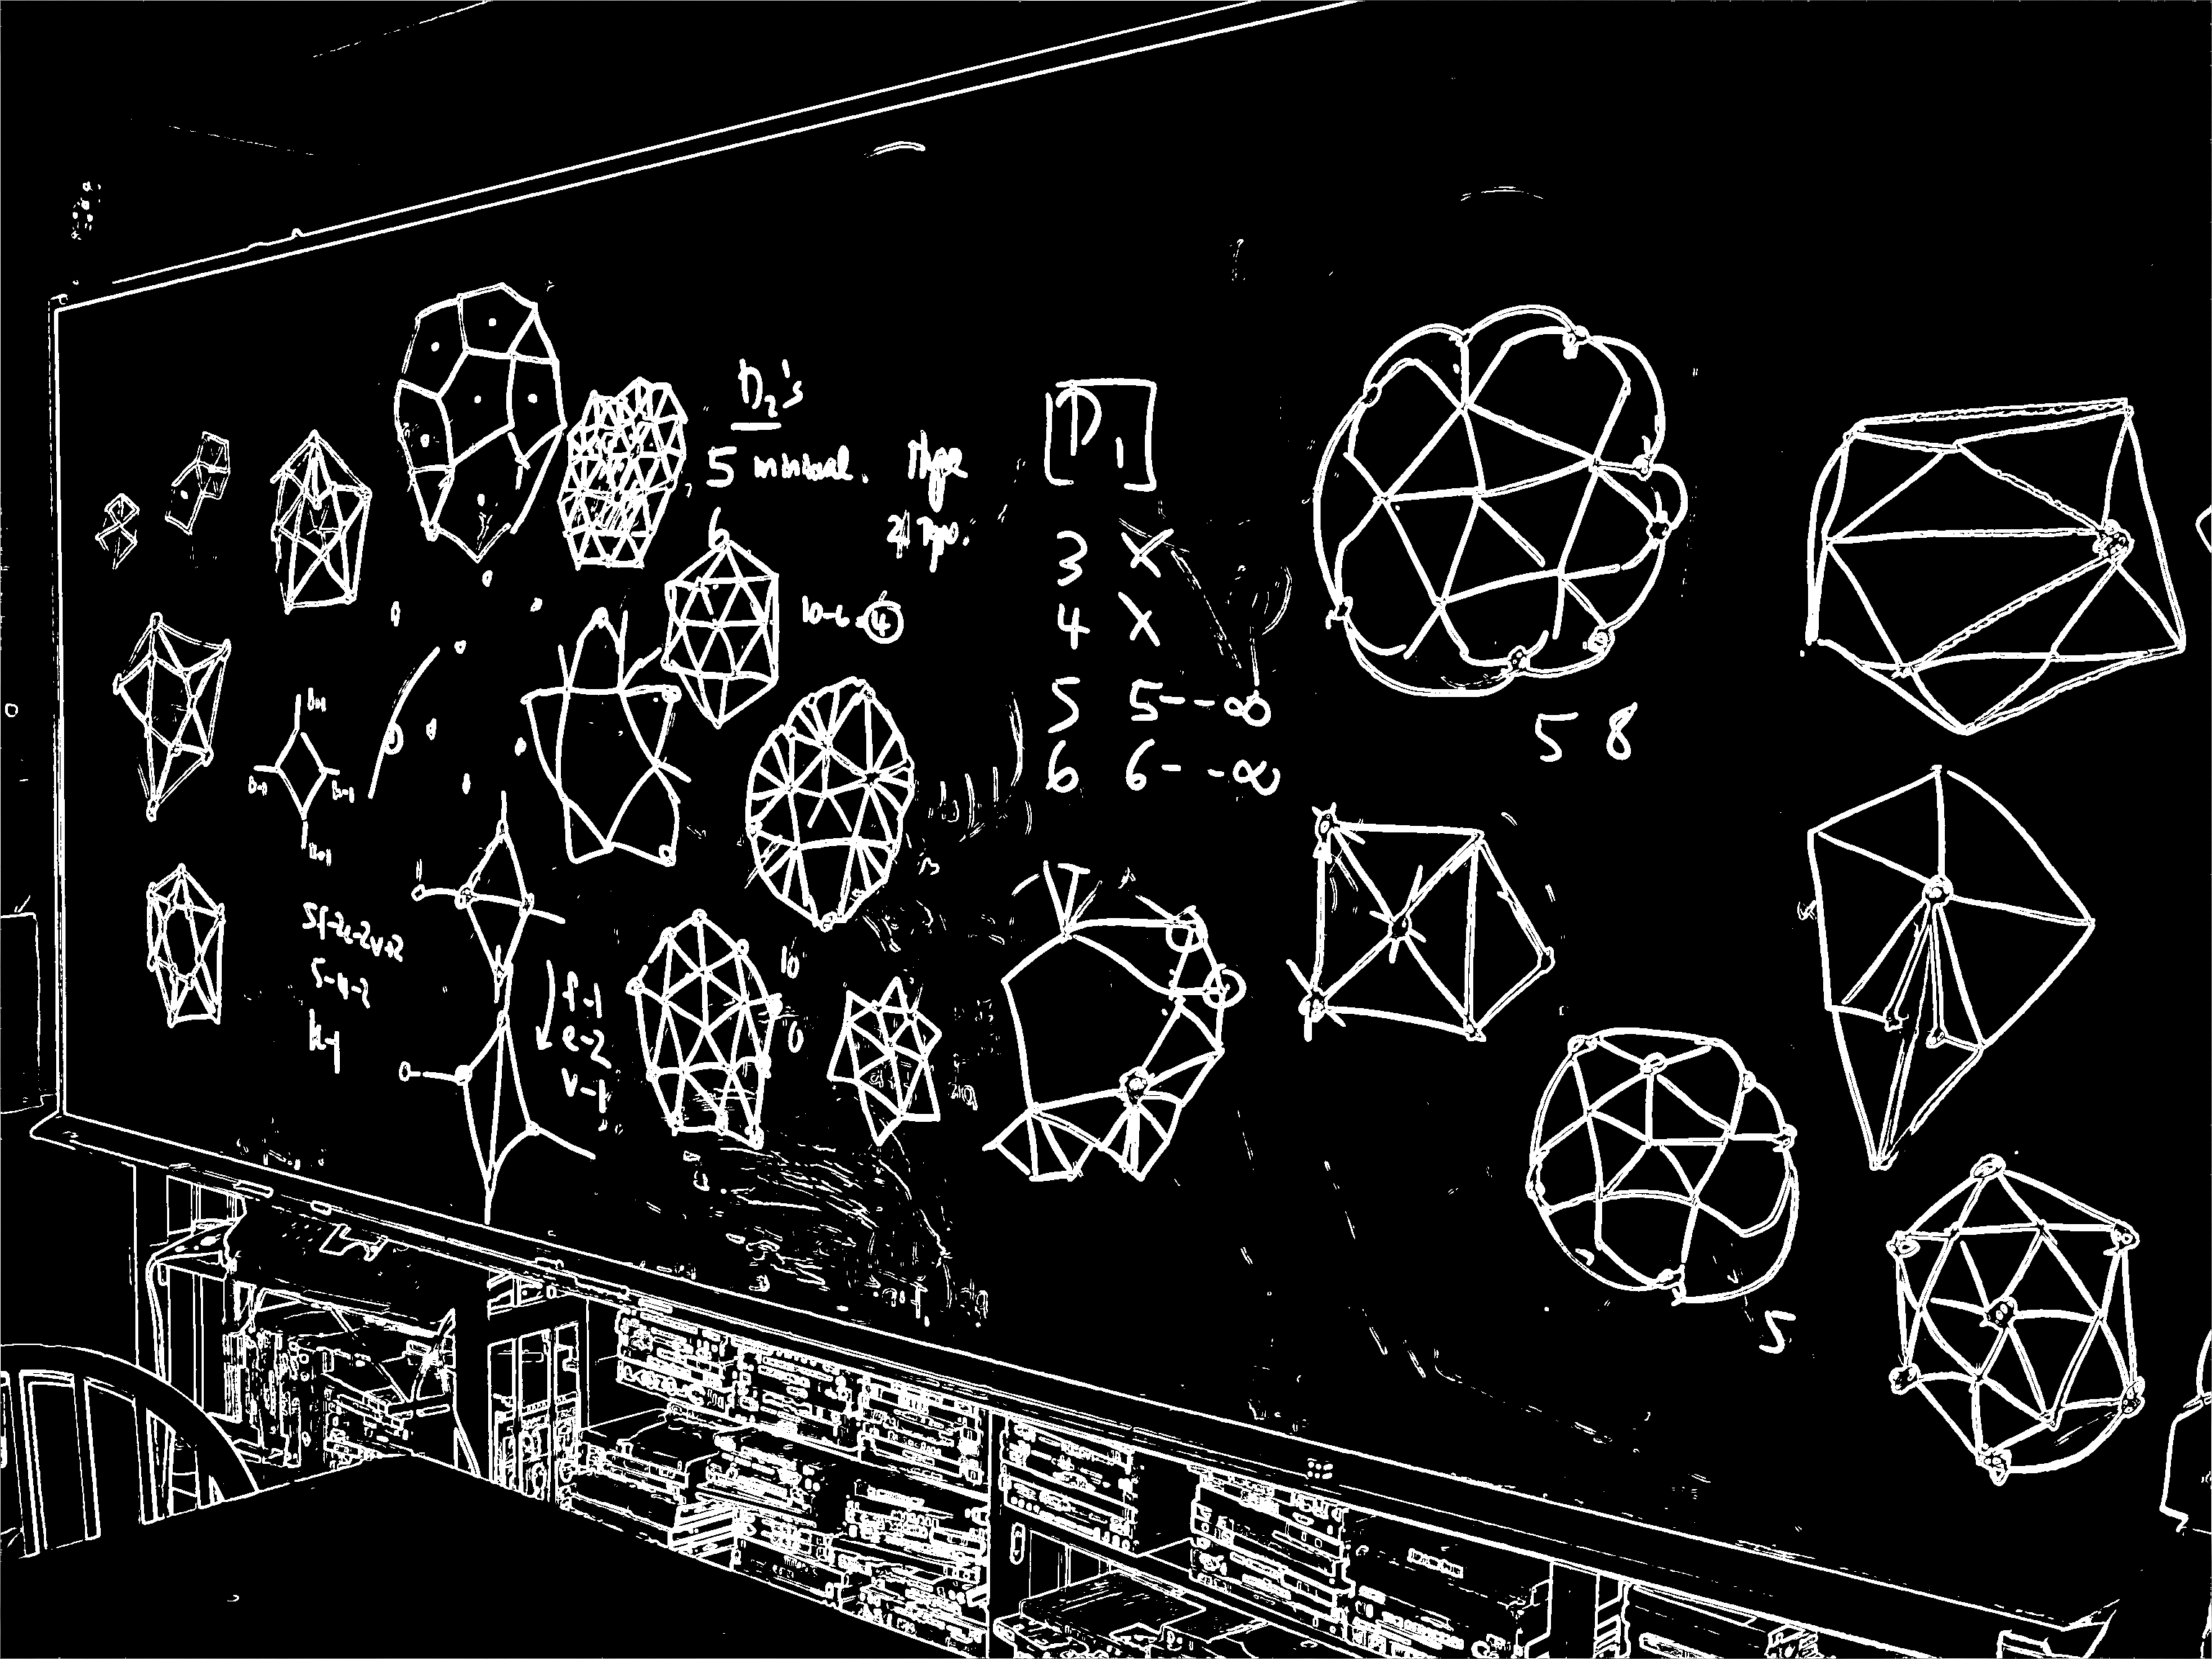
\includegraphics[width=5cm]{images/blackboard_25.png}
  \caption{threshold = 0.25}
\end{figure}
\columnbreak
% second column
\begin{figure}[H]
\centering
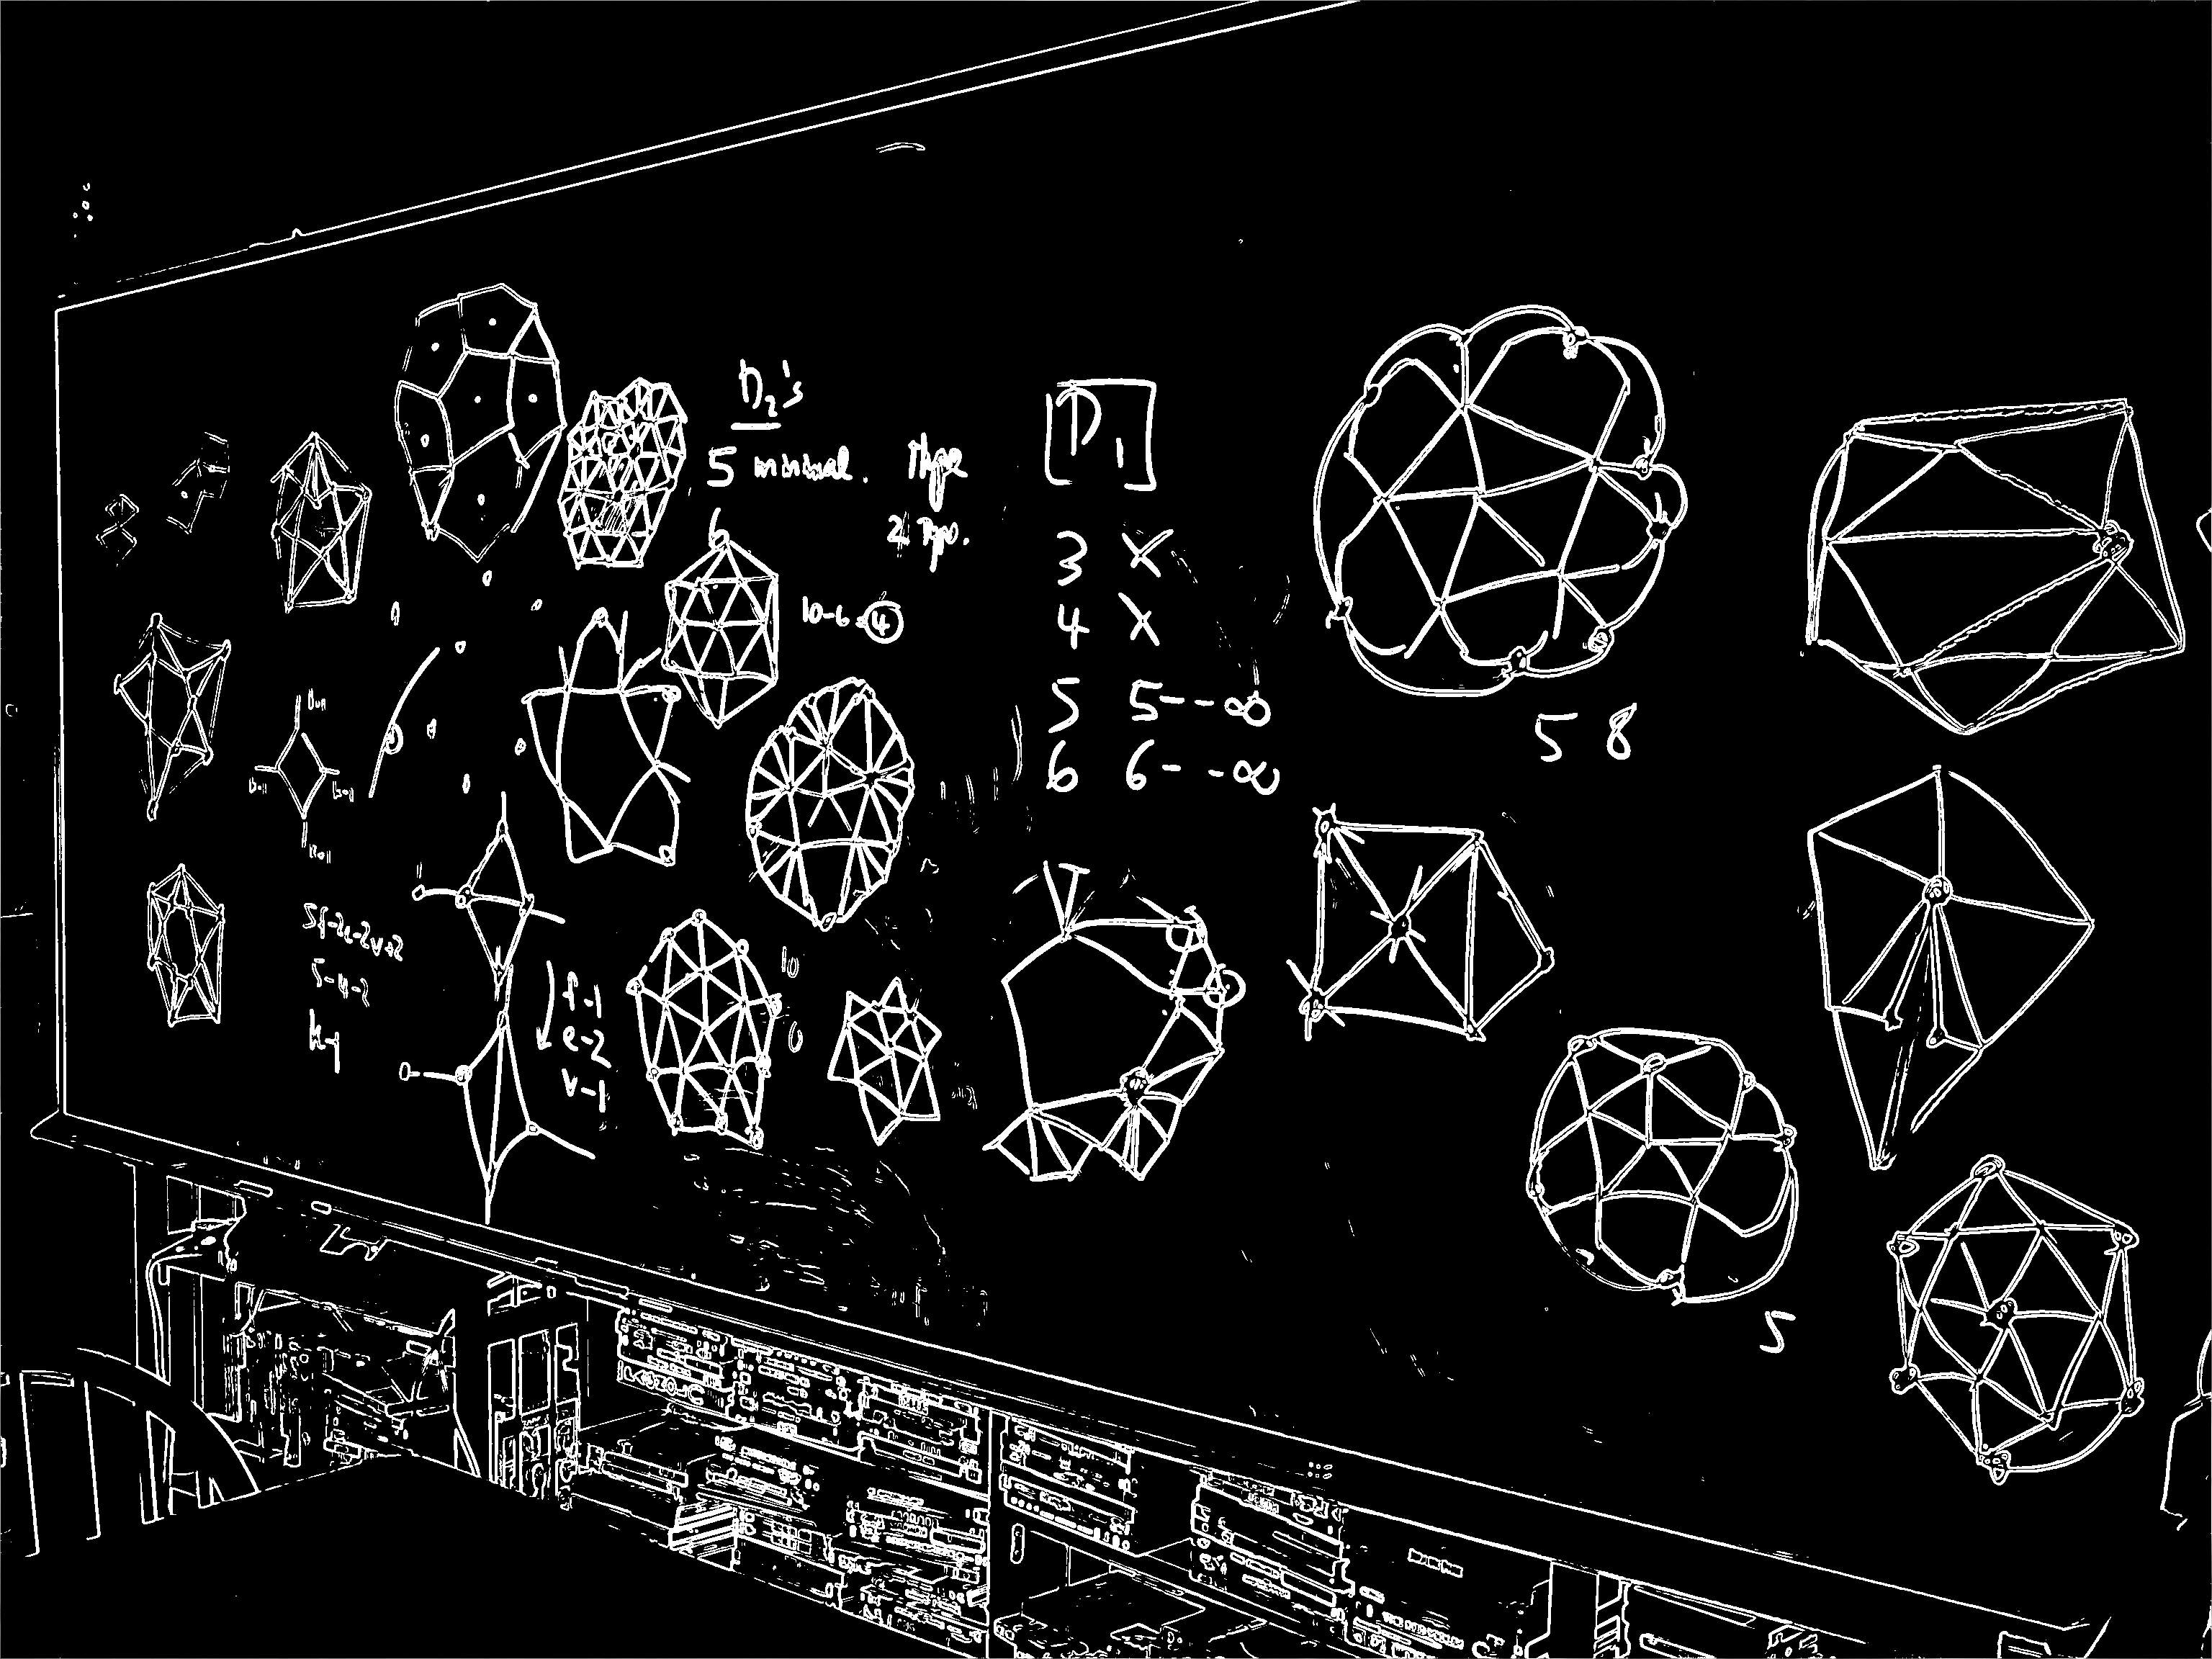
\includegraphics[width=5cm]{images/blackboard_35.png}
  \caption{threshold = 0.35}
\end{figure}
\columnbreak
% third column
\begin{figure}[H]
\centering
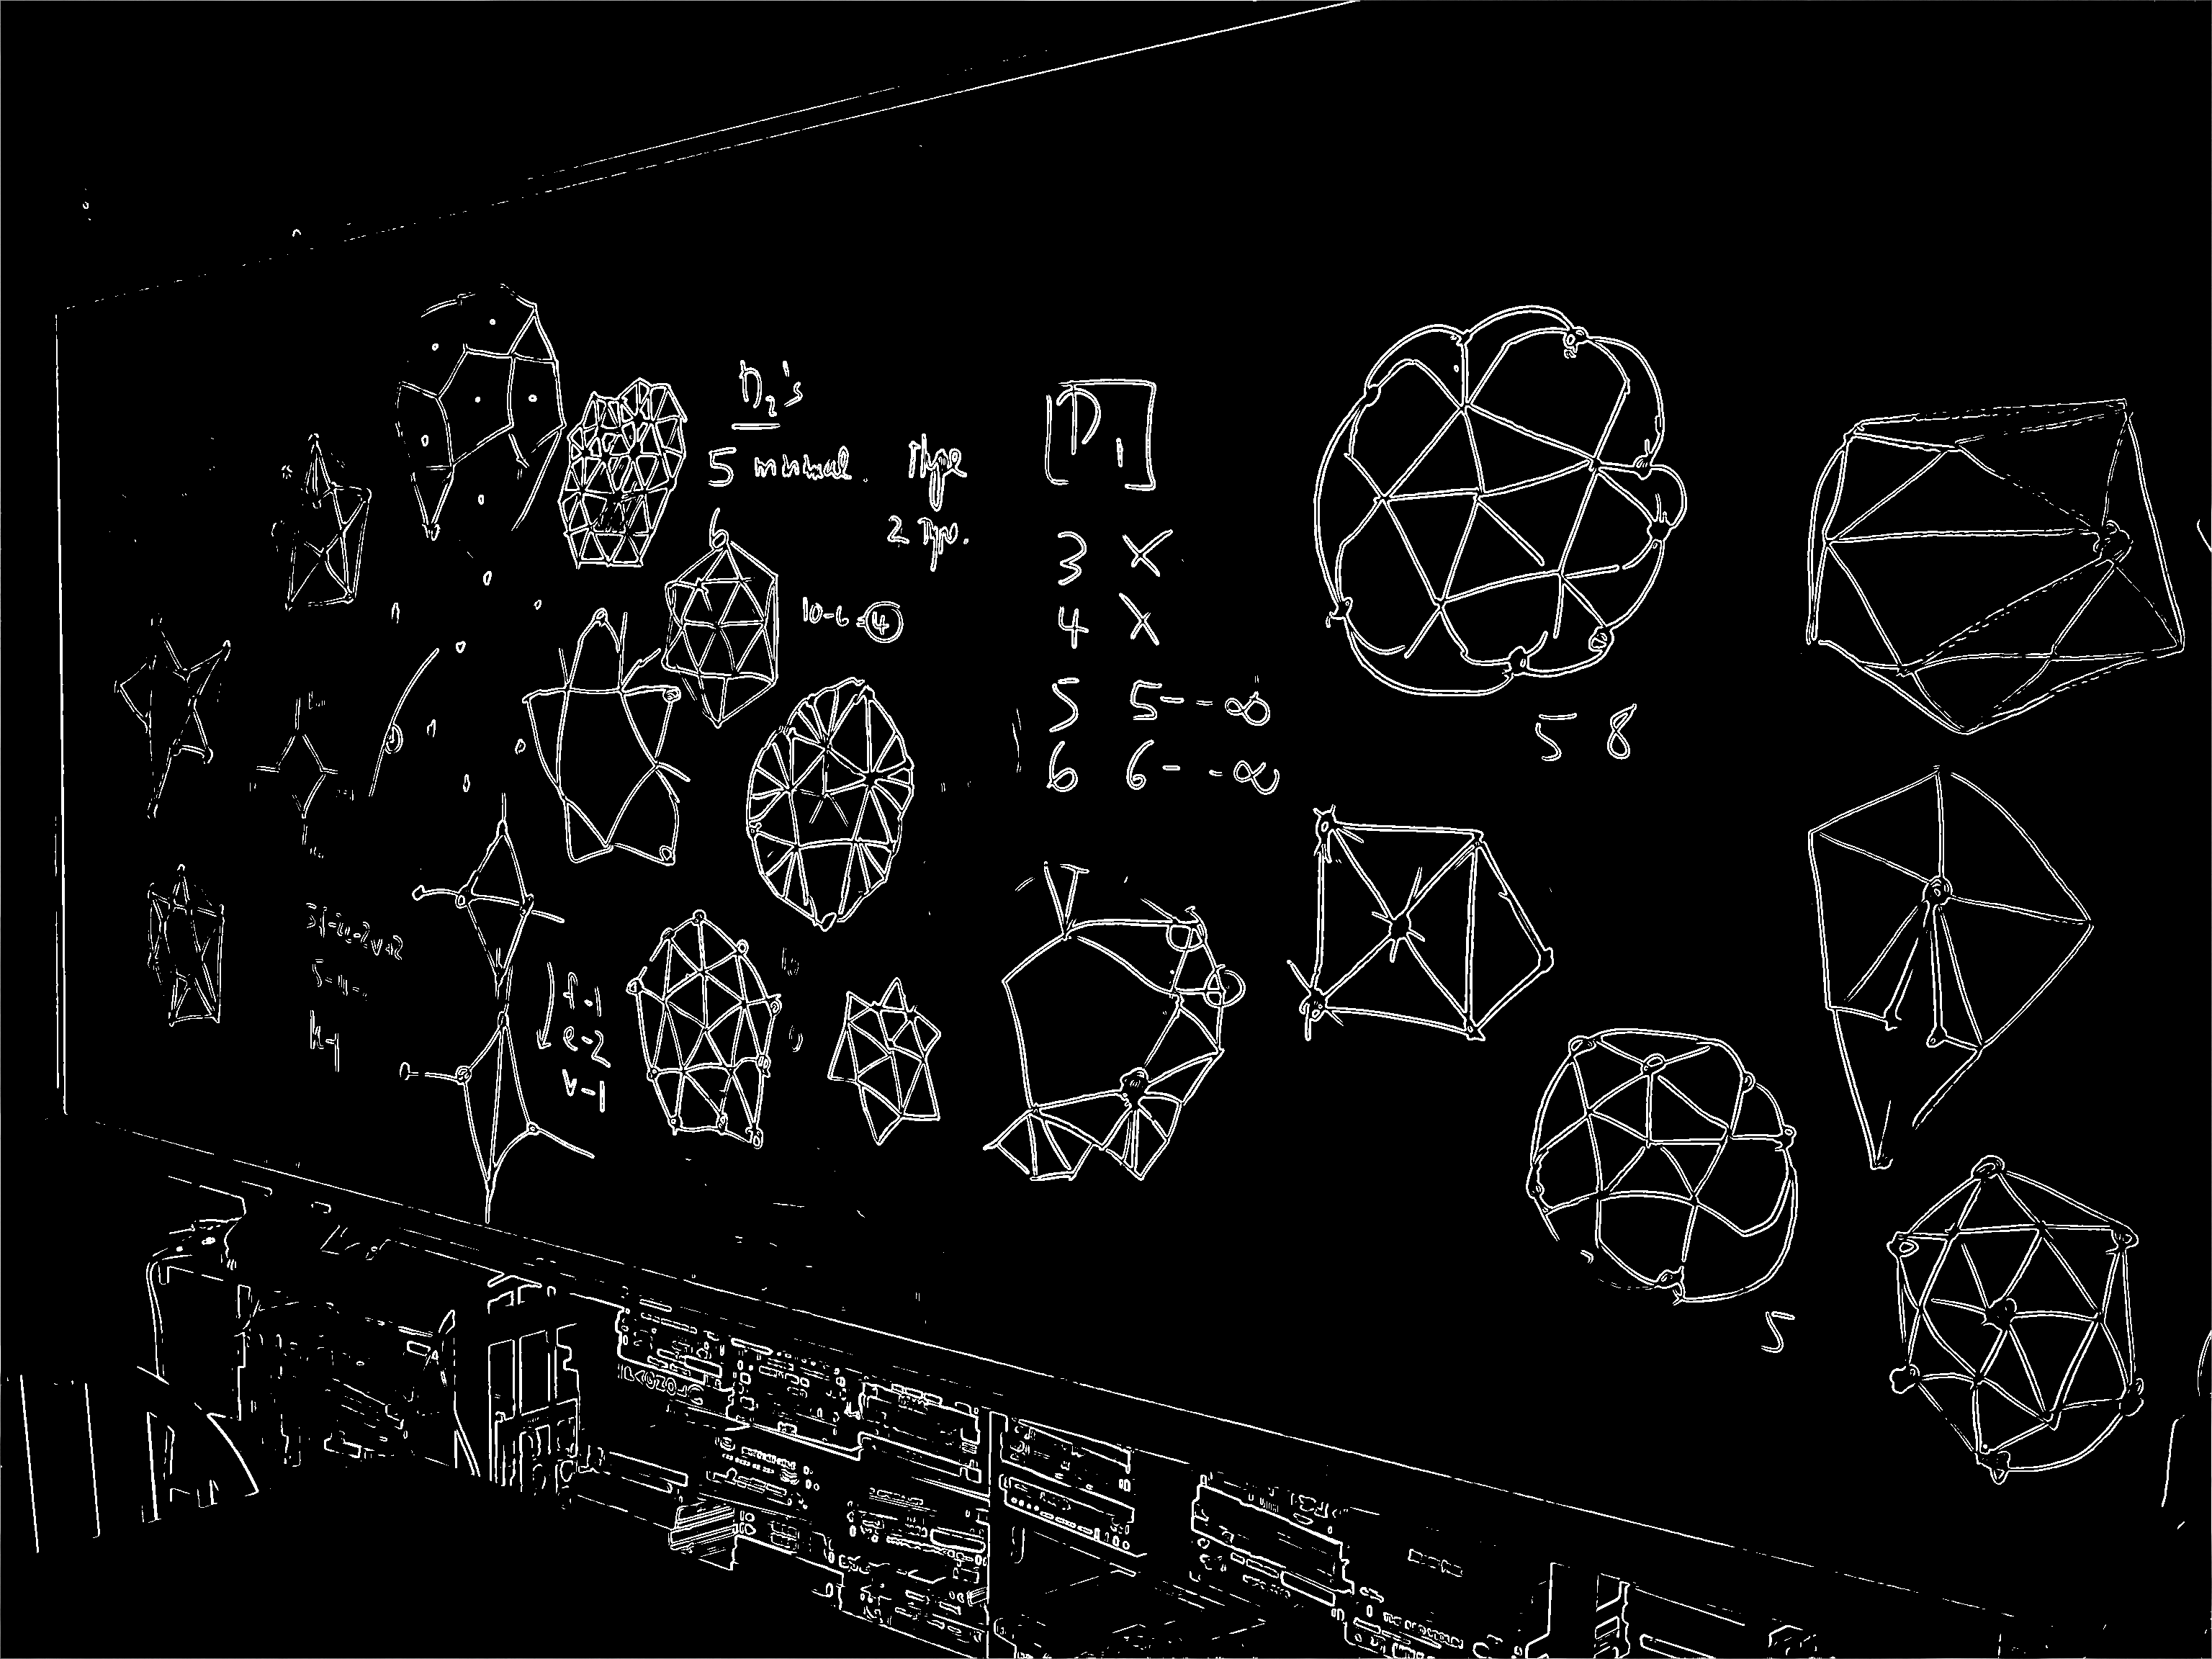
\includegraphics[width=5cm]{images/blackboard_5.png}
  \caption{threshold = 0.5}
\end{figure}
\end{multicols}

\subsection{FED i CED}

Na Slikama \ref{fed_output} i \ref{canny_output} mo\v zemo videti izlaze ovih algoritama.

\begin{multicols}{2}
% first column
\begin{figure}[H]
\centering
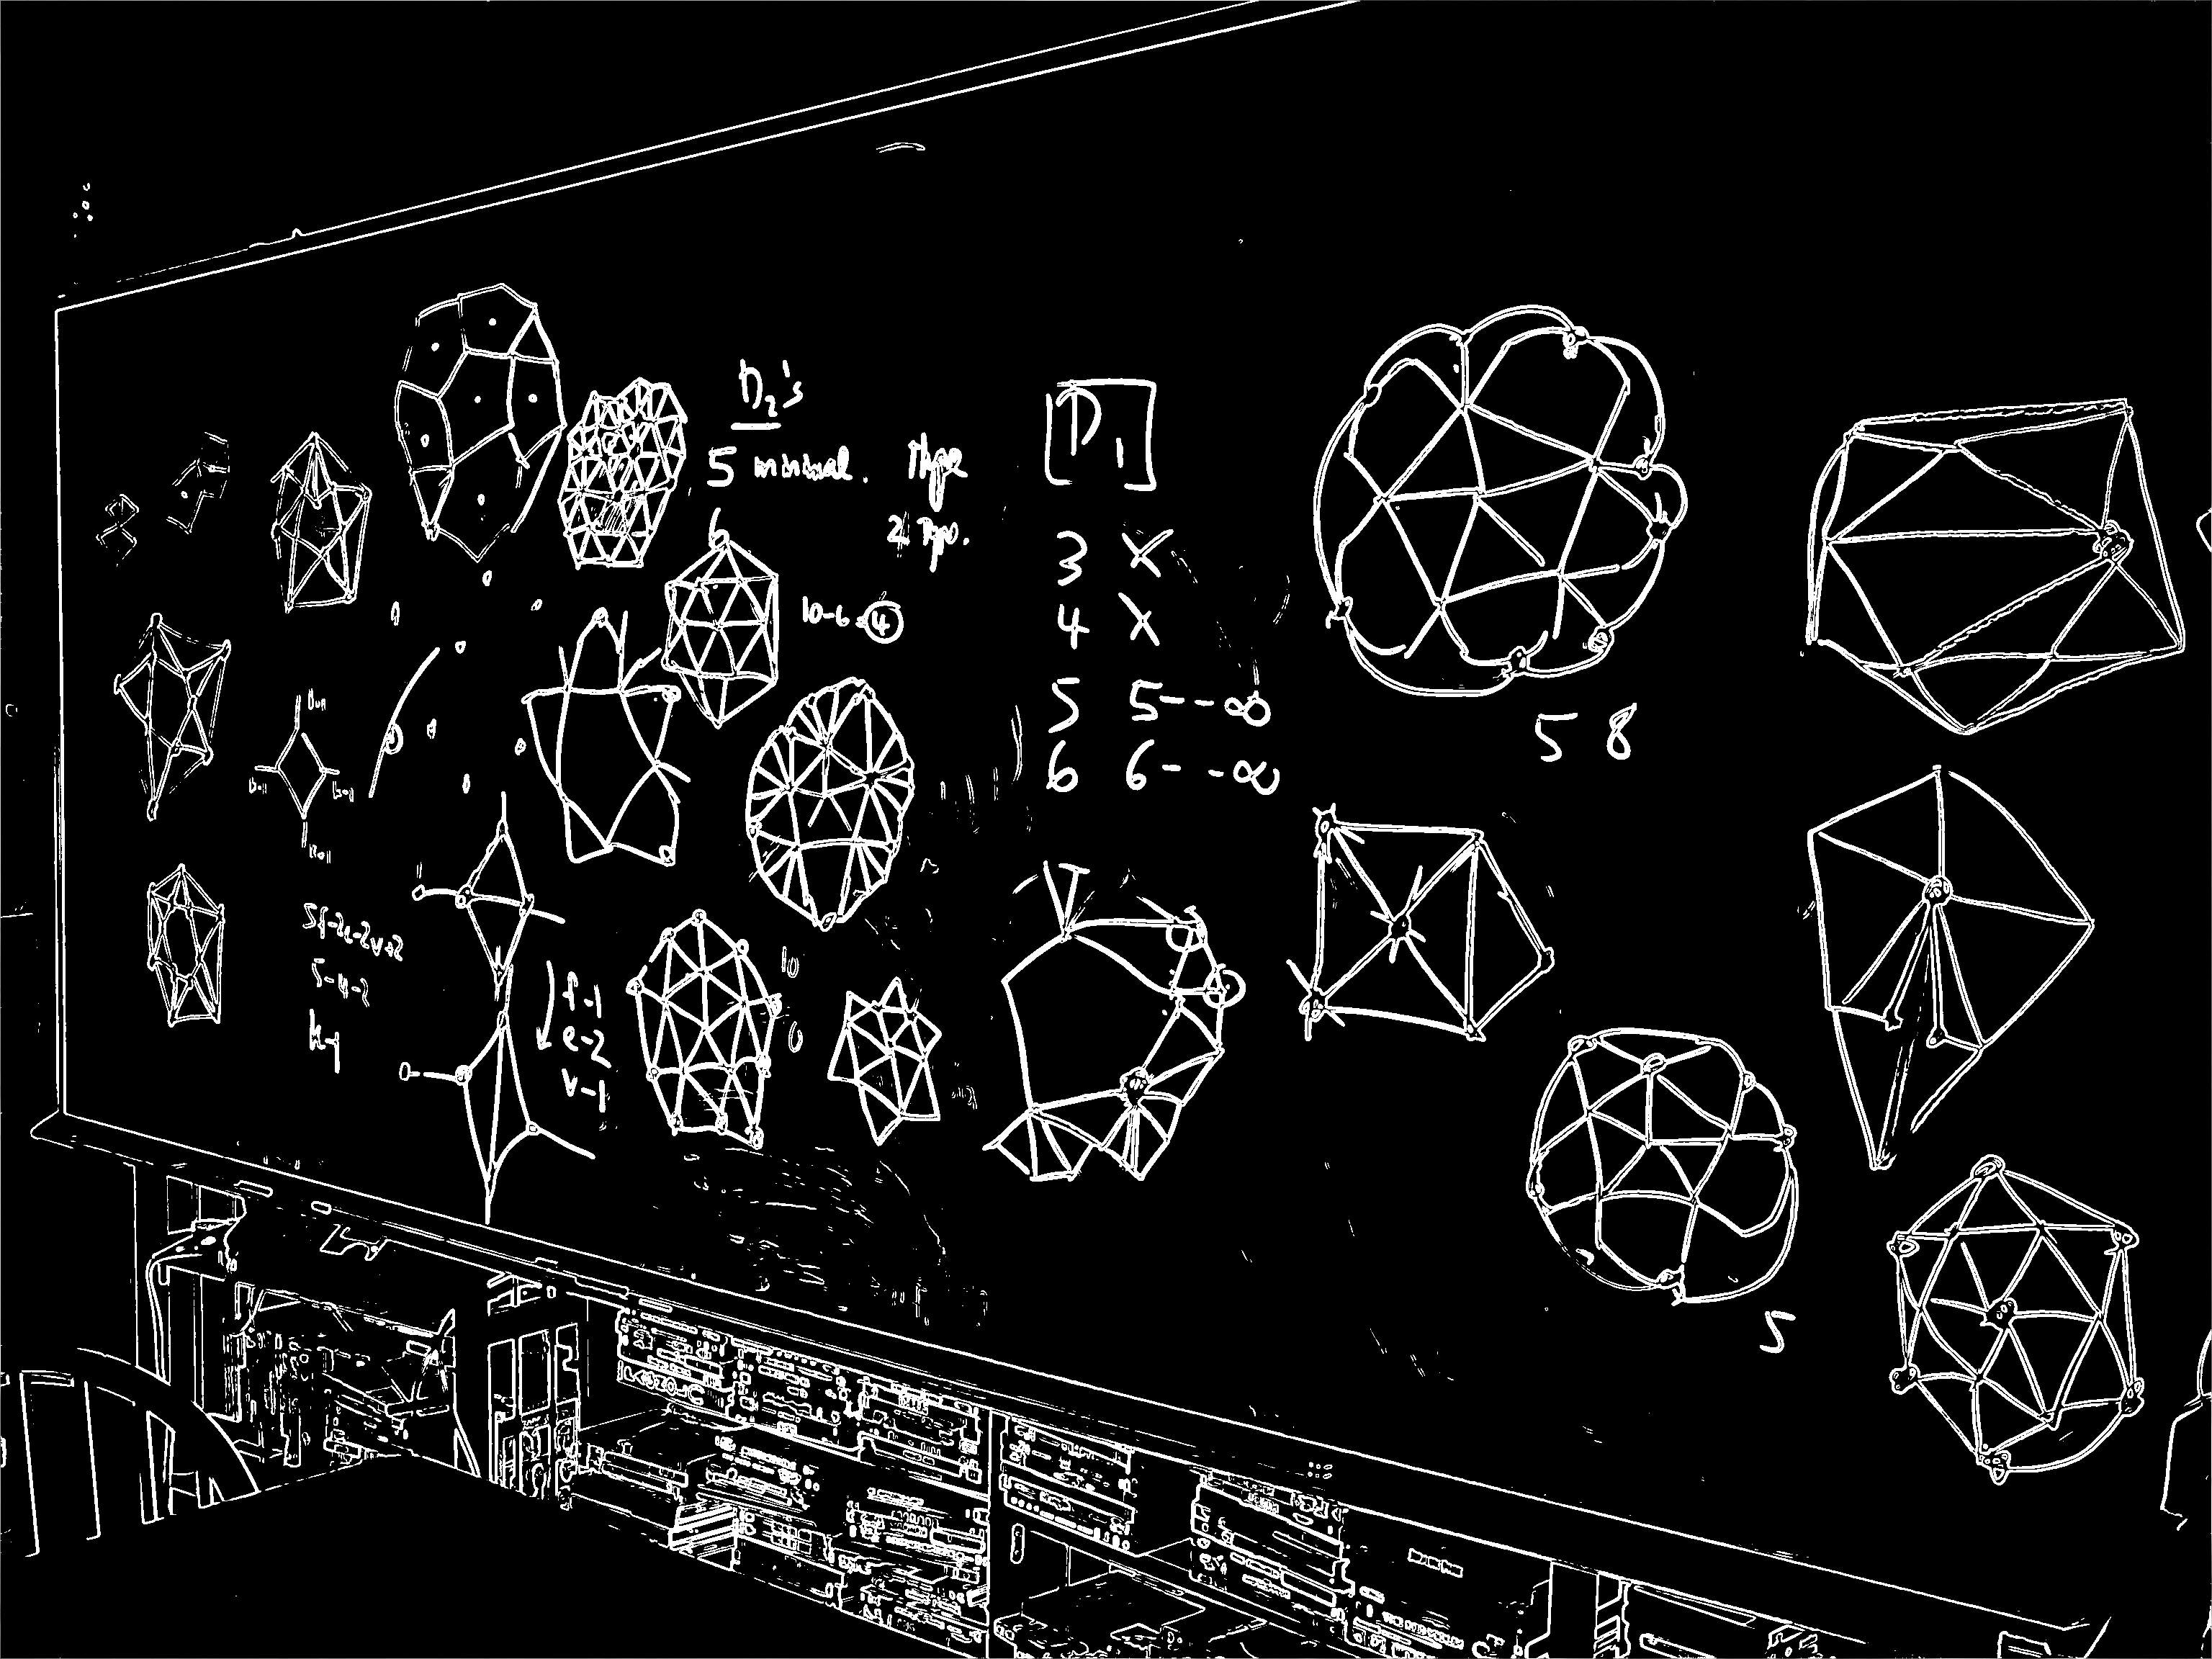
\includegraphics[width=7cm]{images/blackboard_35.png}
  \caption{FED output}\label{fed_output}
\end{figure}

\columnbreak

\begin{figure}[H]
\centering
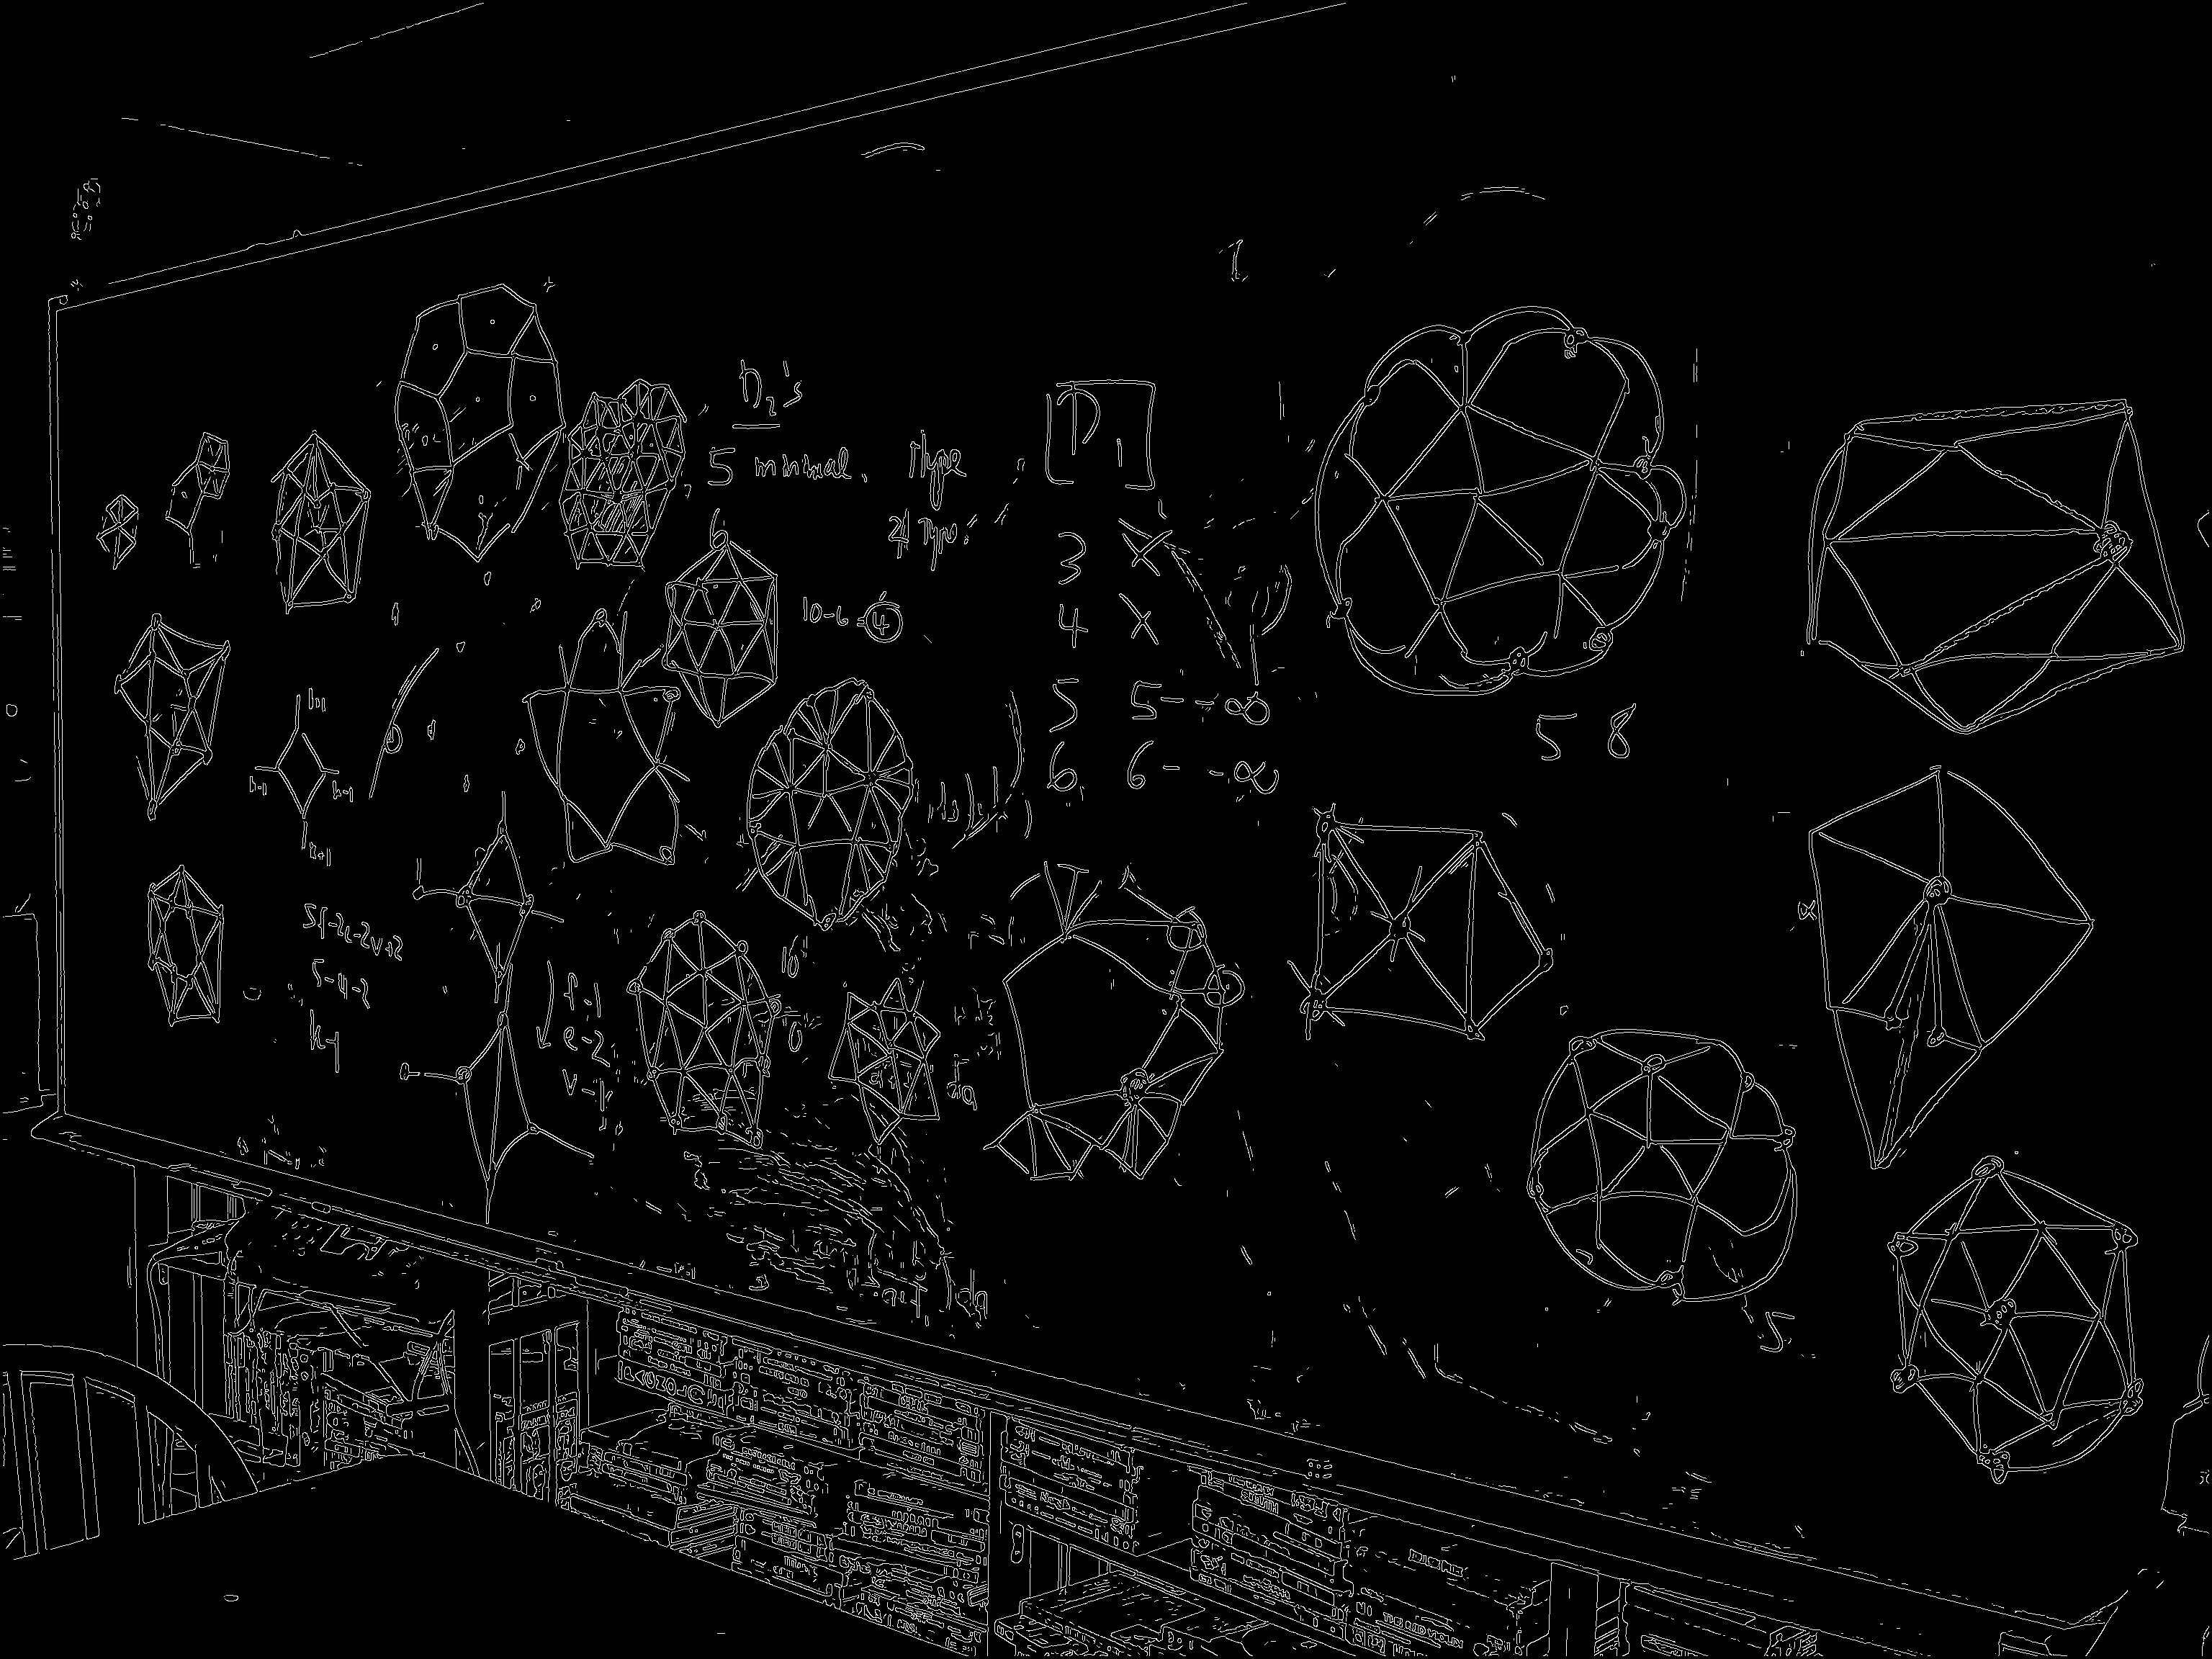
\includegraphics[width=7cm]{images/blackboard_canny.png}
  \caption{Canny output}\label{canny_output}
\end{figure}
\end{multicols}

Iako naizgled izgleda da FED daje bolje rezultate, ivice kod Canny algoritma su tanje (\v sto je po\v zeljno) i to mo\v zemo videti tako \v sto \' cemo prikazati uve\' cane delove Slika \ref{fed_output} i \ref{canny_output}.

\begin{multicols}{2}
% first column
\begin{figure}[H]
\centering
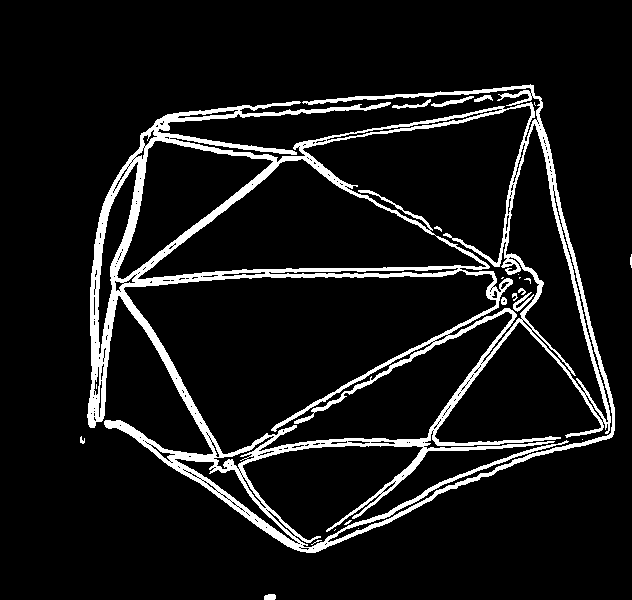
\includegraphics[width=7cm]{images/fuzzy.png}
  \caption{FED output}
\end{figure}

\columnbreak

\begin{figure}[H]
\centering
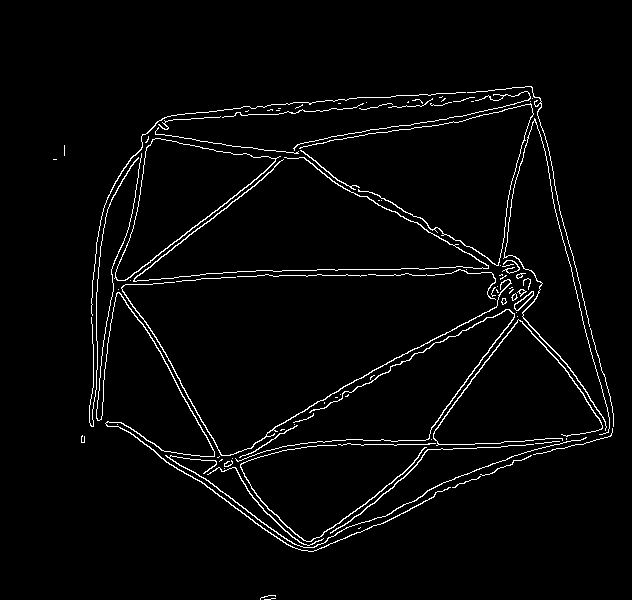
\includegraphics[width=7cm]{images/canny.png}
  \caption{Canny output}
\end{figure}
\end{multicols}

U pore\dj enju sa CED, FED je dosta br\v zi. Naime, za obradu Slike \ref{blackboard_fed_input} sto puta, FED algoritmu je bilo potrebno 60 sekundi, dok CED algoritmu 110. Naravno, ograni\v cavamo se na ru\v cnu implementaciju CED-a autora koja je najverovatnije sporija od implementacije istog algoritma u bibliotekama.\\

Jo\v s jedna prednost FED u odnosu na CED je to \v sto se mnogo lak\v se implementira.


\section{Ulep\v savanje slika kori\v s\v cenjem fazi logike}

Ulep\v savanje slika (eng. image enhancement) predstavlja jedan od osnovnih zadataka obrade slika. \\
Cilj je obraditi ulaznu sliku tako da izlazna bude pogodnija od ulazne za neku specifi\v cnu upotrebu. 

Slike sa lo\v sim kontrastom, lo\v se osvetljene i zamu\' cene slike se dobijaju usled nesavr\v senosti uredjaja koji ih prave (senzori, fotoaparati, itd.), neodgovaraju\' cih uslova za vreme pravljenja slike (lo\v se svetlo) i tokom prenosa slika.
\\ \\
Sa druge strane, slike sa dobrim kontrastom, dobro osvetljene slike, one koje daju dovoljno informacija posmatra\v cu, potrebne su za veliki broj drugih oblasti (medicina, analiza prostora, autonomna navigacija, obrada slika dobijenih satelitima) ili za dalju obradu slika.
\\ \\
Metodi za ulep\v savanje slika se mogu podeliti u 3 grupe [4]:
\\
\\1. Prostorni metod (eng. spatial domain method)
\\2. Metod domena frekvencija (eng. frequency domain method)
\\3. Fazi metod (eng. fuzzy method)
\\ \\ 
Prostorni metodi primenjuju odredjenu transformaciju nad svakim pikselom slike. Daju dosta dobre rezultate, ali se mo\v ze desiti da rezultuju\' ca slika ne izgleda uvek adekvatno (npr. da izgleda isprano).
Neke od prostornih metoda zasnivaju svoj rad na histogramu slike (pomeranje histograma (eng. histogram sliding), razvla\v cenje histograma (eng. histogram stretching), pode\v savanje histograma (eng. histogram equalization)).
Rezultati metoda pode\v savanja histograma \' ce biti poredjeni sa rezultatima koje daje predstavljena fazi metoda.
\\ \\ 
Metod domena frekvencija se pokazuje kao dosta skup [3], \v cak i uz kori\v s\' cenje brzih transformacija (npr. brza Furijeova transformacija), tako da nije pogodan za obradu slika u realnom vremenu.
\\ \\ 
Fazi metod je sposoban da imitira pona\v sanje eksperta uz kori\v s\' cenje baze znanja.\\
Postoji veliki broj metoda koji kombinuje metodu pode\v savanja histograma sa metodom zasnovanom na fazi logici.
Mnoge fazi metode prate standardan sled koraka (fazifikacija, promena vrednosti funkcije pripadnosti, defazifikacija), dok neke ne prolaze kroz sve ove korake.
\\
\\
U nastavku su predstavljene 2 metode za ulep\v savanje slika zasnovane na fazi logici: jedna za slike u boji, druga za crno-bele slike.

\newpage
\subsection{Tehnika za ulep\v savanje crno-belih slika sa lo\v sim kontrastom [3]}

Vrednosti ulazne slike $X$, dimenzija M x N, fazifikuju se primenom funkcije $\mu$:\\
\begin{align*}
  \mu_{ij} = \mu(x_{ij}) =  \frac{x_{ij} - x_{min}}{x_{max} - x_{min}}\\ \\
  0\leq i \leq M, 0\leq j \leq N
\end{align*}
$x_{max}$, $x_{min}$ predstavljaju maksimalnu i minimalnu vrednost piksela koja se mo\v ze na\' ci na slici $X$, respektivno.\\
$x_{ij}$ predstavlja vrednost piksela na mestu $ij$ slike $X$. Za 8-bitnu sliku, ta vrednost mo\v ze biti u intervalu $[0, 2^8 - 1]$. \\ 
$\mu_{ij}$ predstavlja stepen osvetljenosti koju ima piksel $ij$ na ulaznoj slici $X$. U fazi terminologiji, $\mu$ je funkcija pripadnosti i omogu\' cava 
prevodjenje nefazi ulaza (slika $X$) u njen odgovaraju\' ci fazi oblik.
Stoga, $0\leq \mu_{ij} \leq 1$.\\

Kako bi se dobio \v sto bolji rezultat, za modifikaciju funkcije pripadnosti se uzima poznati INT operator, koji su predlo\v zili King i Pal 1981. godine [5].\\

INT operator primenjen na vrednostima funkcije pripadnosti $\mu$: \\

\[
  \bar\mu_{ij}(\mu_{ij}) = 
    \begin{cases} 
      2 * \mu_{ij}^2 & 0\leq \mu_{ij}\leq \mu_{c} \\
      1 - (2 * (1 - \mu_{ij})^2) & \mu_{c}\leq \mu_{ij}\leq 1 
    \end{cases}
 \]

Ta\v cka $\mu_{c}$ je grani\v cna vrednost koja se mo\v ze menjati. Naj\v ce\v s\' ce uzimana vrednost za nju je $0.5$ 
(takodje kori\v s\' cenja i u na\v soj implementaciji). \\

Formula kojom je predstavljen INT operator, u stvari, predstavlja matemati\v cku formulaciju
naredna 3 if-then pravila: \\ \\
1. Ako je piksel svetao, onda \'ce biti svetliji.\\
2. Ako je piksel siv, onda \'ce biti siv. \\
3. Ako je piksel taman, onda \'ce biti tamniji.\\ \\
Prakti\v cno, nakon primene INT operatora, vrednost piksela sa funkcijom pripadnosti manjom od 0.5 \' ce se smanjiti. Oni pikseli sa ve\' com vredno\v s\' cu \' 
funkcije pripadnosti od 0.5 ima\' ce ve\' cu vrednost.
\\

Nakon modifikacije funkcije pripadnosti, dobijene vrednosti treba defazifikovati i na taj na\v cin dobiti nove nijanse sive, izlaznu sliku.\\
Izlazna slika $Y$ se dobija primenom inverzne funkcije $\mu^{-1}$:\\
\begin{align*}
  y_{ij} = \mu^{-1}(\bar\mu_{ij})\\
  y_{ij} = x_{min} + \bar\mu * (x_{max} - x_{min})
\end{align*}

\inputminted[tabsize=2,breaklines]{cpp}{codes/latex/fuzzy_grayscale.cpp}

Na Slici \ref{tree_fuzzy_grayscale_output}, \ref{fuzzy_grayscale_output1} i \ref{fuzzy_grayscale_output2} su prikazani rezultati rada algoritma.

\begin{multicols}{2}
% first column
\begin{figure}[H]
\centering
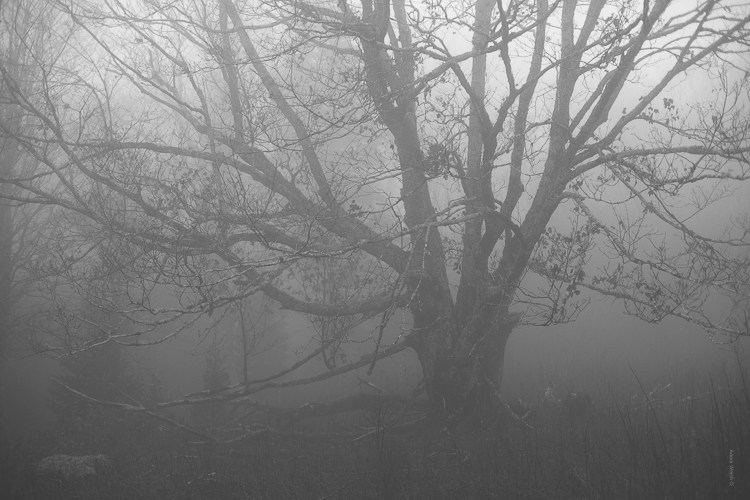
\includegraphics[width=8cm]{images/tree.jpg}
  \caption{Original}\label{tree_fuzzy_grayscale_input}
\end{figure}
\columnbreak
% second column
\begin{figure}[H]
\centering
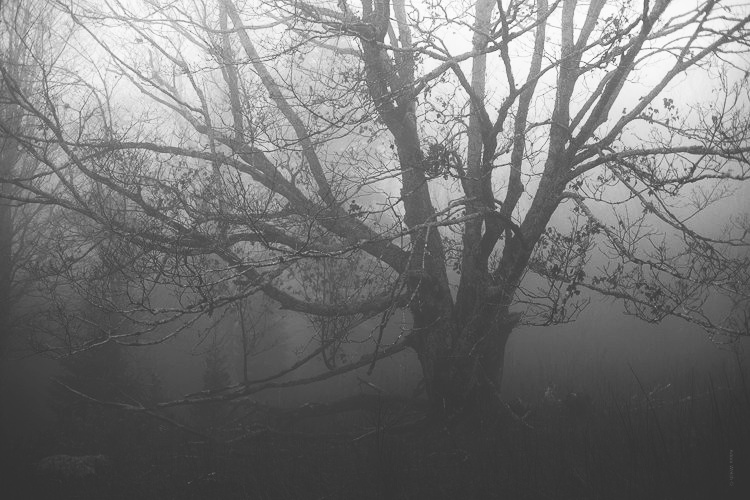
\includegraphics[width=8cm]{images/fuzzy_grayscale_0.jpg}
  \caption{Rezultat}\label{tree_fuzzy_grayscale_output}
\end{figure}
\end{multicols}

\newpage

\begin{multicols}{2}
% first column
\begin{figure}[H]
\centering
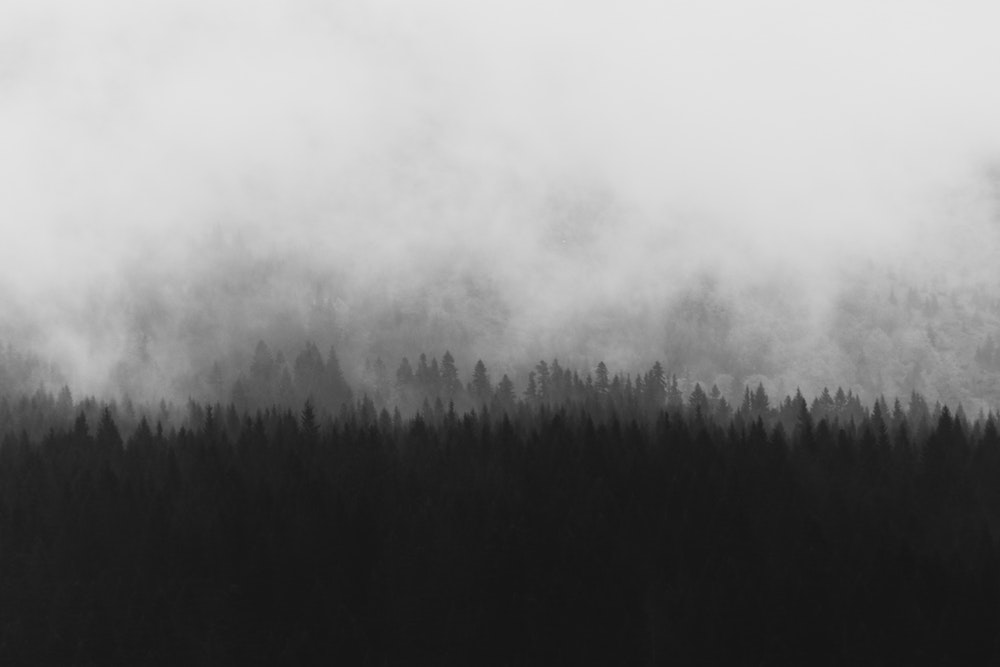
\includegraphics[width=8cm]{images/wood.jpeg}
  \caption{Original}\label{tree_fuzzy_grayscale_input}
\end{figure}
\columnbreak
% second column
\begin{figure}[H]
\centering
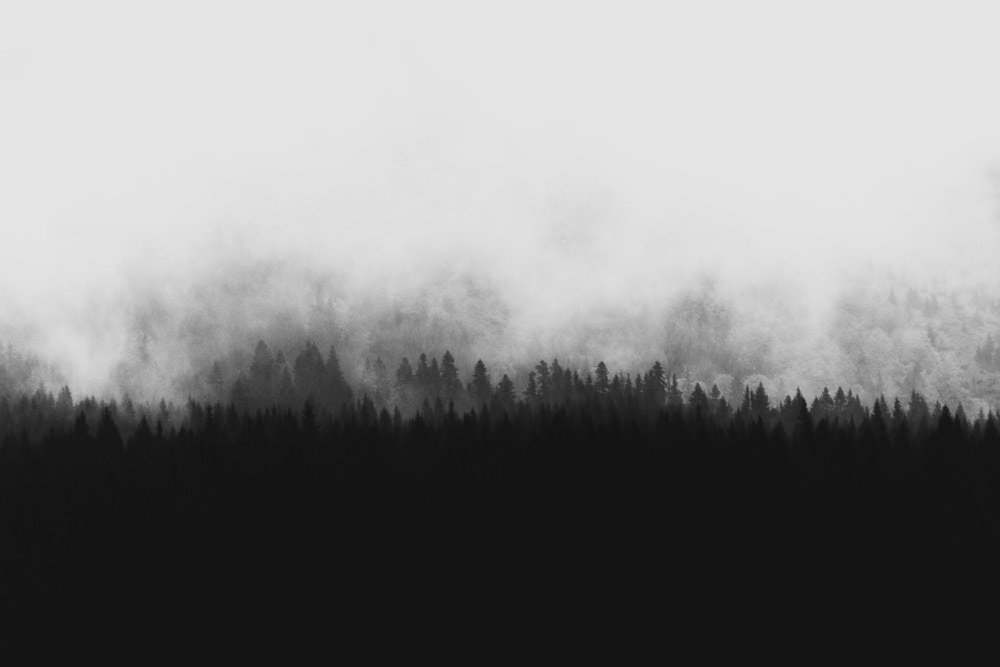
\includegraphics[width=8cm]{images/fuzzy_grayscale_1.jpg}
  \caption{Rezultat}\label{fuzzy_grayscale_output1}
\end{figure}
\end{multicols}

\begin{multicols}{2}
% first column
\begin{figure}[H]
\centering
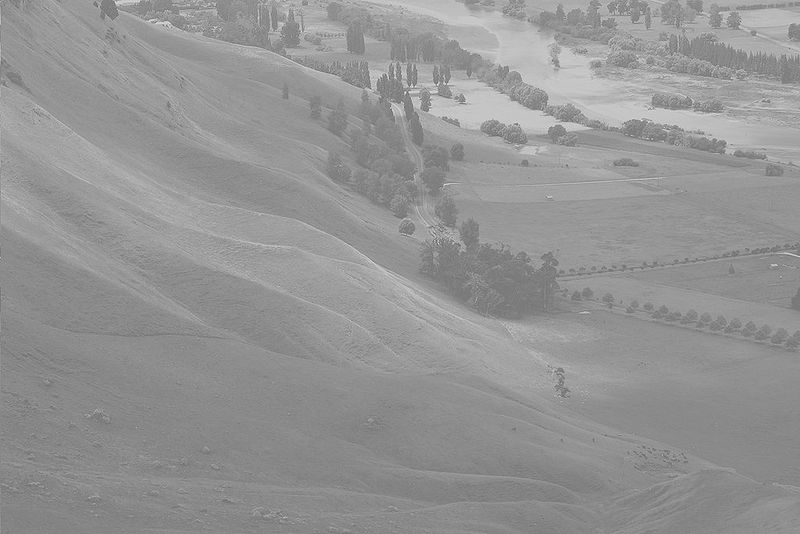
\includegraphics[width=8cm]{images/field.jpg}
  \caption{Original}\label{tree_fuzzy_grayscale_input}
\end{figure}
\columnbreak
% second column
\begin{figure}[H]
\centering
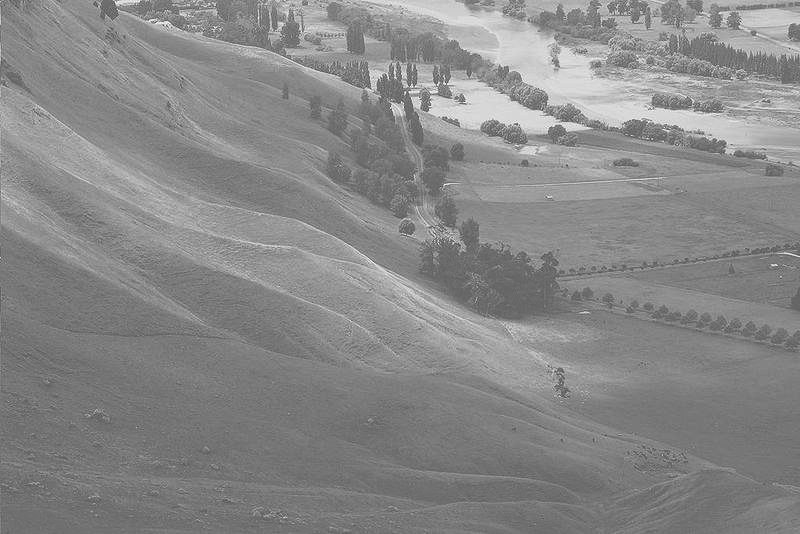
\includegraphics[width=8cm]{images/fuzzy_grayscale_2.jpg}
  \caption{Rezultat}\label{fuzzy_grayscale_output2}
\end{figure}
\end{multicols}

\newpage
\subsection{Tehnika za ulep\v savanje slika u boji sa lo\v sim kontrastom [4]}

RGB model boja je aditivni model boja koji opisuje boju dodavanjem odgovaraju\' ceg stepena crvene, zelene i plave boje. Taj stepen, za 8-bitnu sliku, mo\v ze imati vrednosti u intervalu $[0, 2^8 - 1]$. 
Metod opisan u nastavku pobolj\v sava kontrast slike opisane u RGB modelu boja. \\ \\
Fazifikacija, izmena vrednosti funkcije pripadnosti i defazifikacija se rade posebno na svakom kanalu u\v citane slike $X$, dimenzija M x N.

\begin{align*}
  \mu_{ij} = [1 + \frac{x_{max} - x_{ij}}{Fd}]^{-Fe} \\ \\
  0\leq i \leq M, 0\leq j \leq N
\end{align*}

Kako se formula posebno primenjuje nad svakim kanalom slike $X$, $x_{max}$ predstavlja maksimalnu vrednost trenutno tretiranog kanala piksela koja se mo\v ze na\' ci na slici $X$.\\
$x_{ij}$ predstavlja vrednost piksela na poziciji $ij$. \\ 
$\mu_{ij}$ je vrednost funkcije pripadnosti $x_{ij}$, $0\leq \mu_{ij} \leq 1$.\\
$Fe$ je eksponencijalna fazi konstanta (eng. exponential fuzzifier), koja . \\
Eksperimentalno je pokazano da su dobro izabrane vrednosti za Fe 1 i 2 []. \\
U na\v soj implementaciji 
\begin{align*}
  Fe = 2\\
\end{align*}
$Fd$ je koli\v cni\v cka fazi konstanta (eng. denominational fuzzifier), koja . \\
\begin{align*}
  Fd = \frac{x_{max} - x_{mid}}{0.5^{\frac{-1}{Fe}} - 1}
\end{align*}
\\
$x_{mid}$ je srednja vrednost trenutno tretiranog kanala piksela koja se mo\v ze na\' ci na slici $X$. \\ \\
Nakon fazifikacije se vr\v si modifikacija funkcije pripadnosti za svaki kanal svakog piksela kori\v \' cenjem $INT$ operatora definisanog u formuli (\ref{int_operator}).\\
\\
Defazifikacija se vr\v si kori\v s\' cenjem:\\
\begin{align*}
  y_{ij} = \mu^{-1}(\bar\mu_{ij})\\
  y_{ij} = x_{max} - Fd * (\bar\mu_{ij}^{-Fe}) + Fd\\
\end{align*}

$\bar\mu_{ij}$ je rezultat primene INT operatora n\mbox a $\mu_{ij}$. \\
$y_{ij}$ trenutno tretirani kanal piksela koji \' ce \v ciniti izlaznu sliku $Y$.\\
\\
Kombinovanjem novodobijenih vrednosti crvene, zelene i plave boje svakog piksela ulazne slike $X$, dobija se izlazna slika $Y$.

\inputminted[tabsize=2,breaklines]{cpp}{codes/latex/fuzzy_color_latex.cpp}

Na Slici \ref{river_output}, \ref{woman_output} i \ref{cat_output} su prikazani rezultati rada algoritma.

\begin{multicols}{2}
% first column
\begin{figure}[H]
\centering
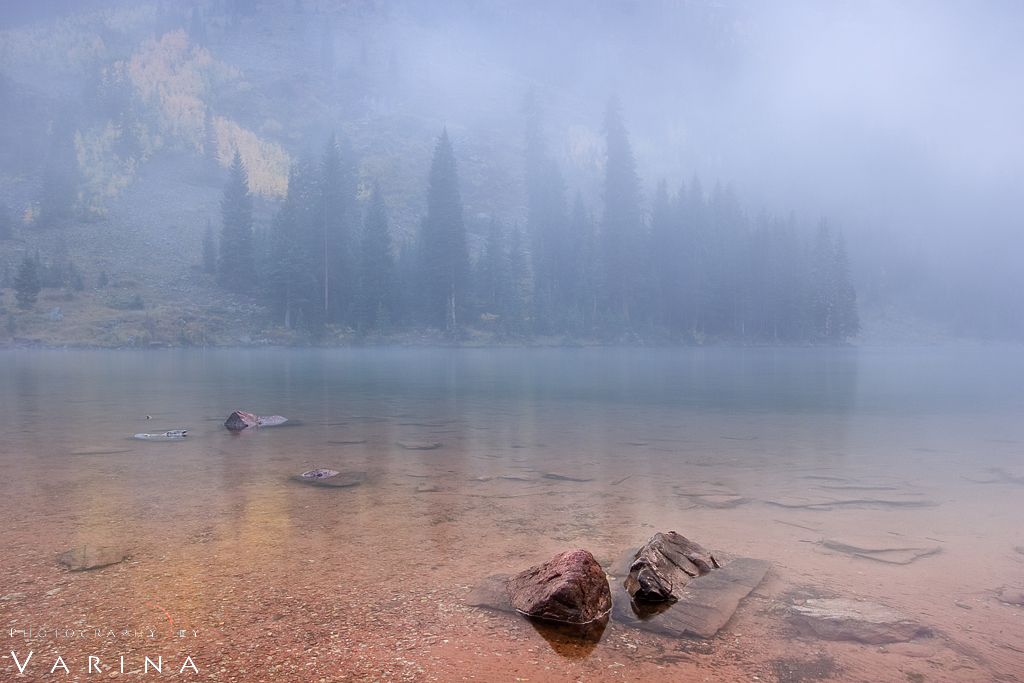
\includegraphics[width=8cm]{images/river.jpg}
  \caption{Original}\label{river}
\end{figure}
\columnbreak
% second column
\begin{figure}[H]
\centering
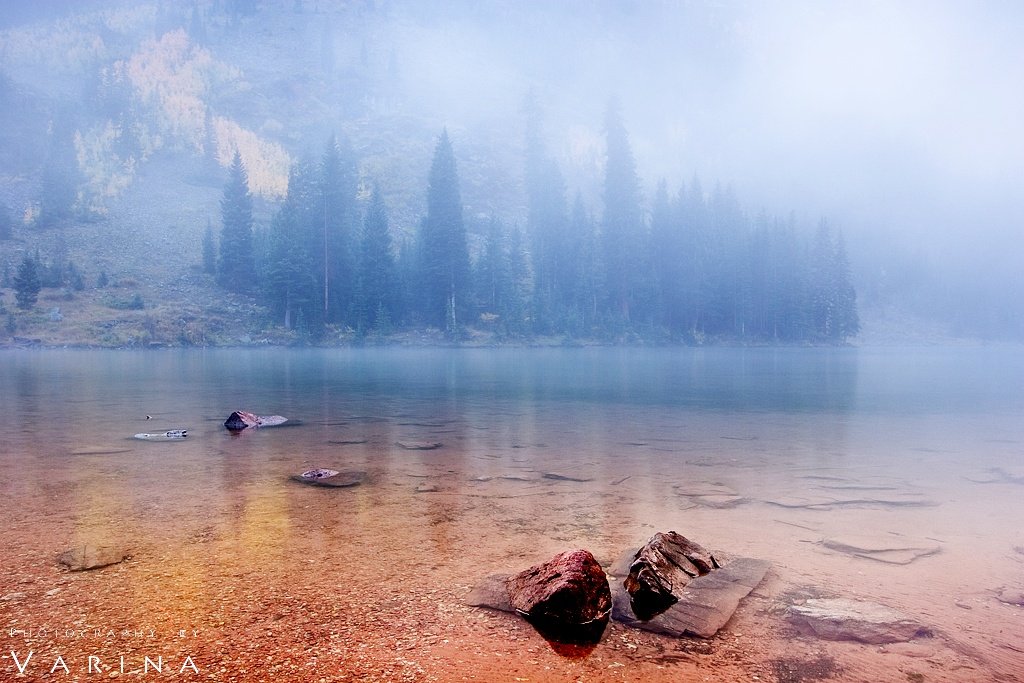
\includegraphics[width=8cm]{images/fuzzy_color_1.jpg}
  \caption{Rezultat}\label{river_output}
\end{figure}
\end{multicols}


\begin{multicols}{2}
% first column
\begin{figure}[H]
\centering
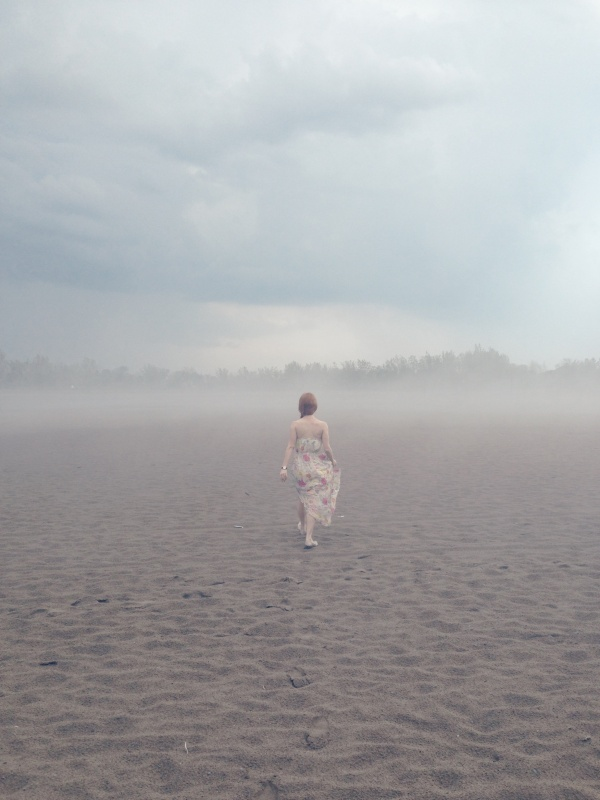
\includegraphics[width=8cm]{images/woman.jpeg}
  \caption{Original}\label{river}
\end{figure}
\columnbreak
% second column
\begin{figure}[H]
\centering
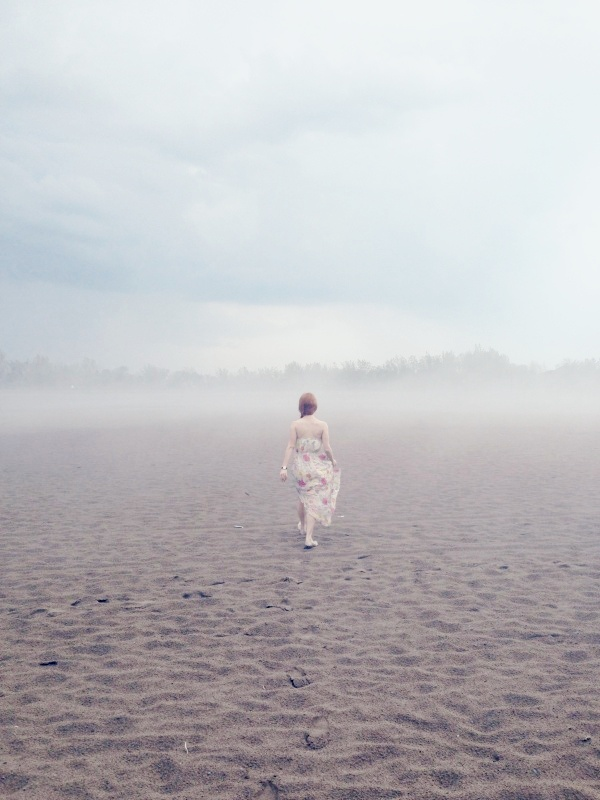
\includegraphics[width=8cm]{images/fuzzy_color_2.jpg}
  \caption{Rezultat}\label{woman_output}
\end{figure}
\end{multicols}

\begin{multicols}{2}
% first column
\begin{figure}[H]
\centering
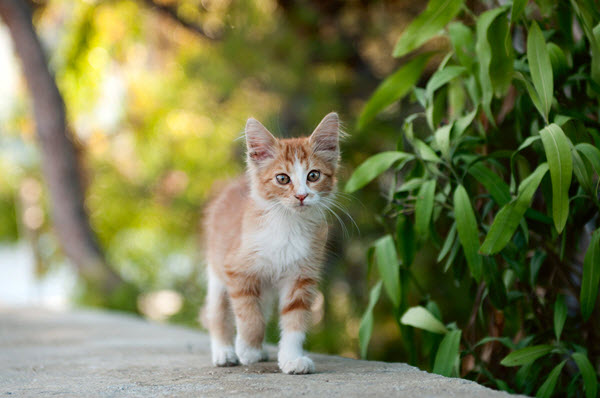
\includegraphics[width=8cm]{images/cat.jpg}
  \caption{Original}\label{river}
\end{figure}
\columnbreak
% second column
\begin{figure}[H]
\centering
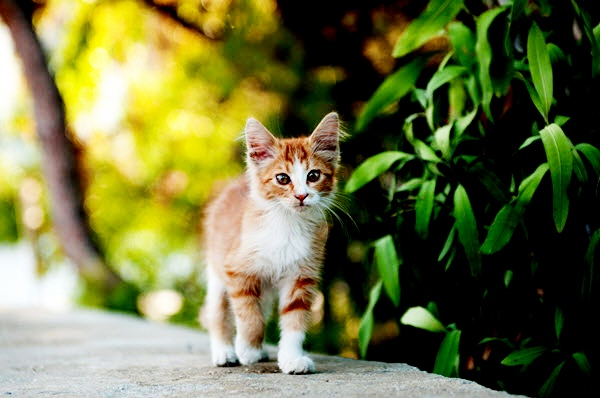
\includegraphics[width=8cm]{images/fuzzy_color_5.jpg}
  \caption{Rezultat}\label{cat_output}
\end{figure}
\end{multicols}

\newpage
\subsection{Poredjenje rezultata metoda za ulep\v savanje slika u boji, crno-belih slika i metoda pode\v savanja histograma}
Metoda pode\v savanja histograma (eng. histogram equalization - HE) je jedna od najpopularnijih metoda za obradu slika. 
Zbog toga \v sto su njeni rezultati dobri, uporedjeni su sa rezultatima predstavljenih fazi metoda. \\  

\begin{multicols}{2}
% first column
\begin{figure}[H]
\centering
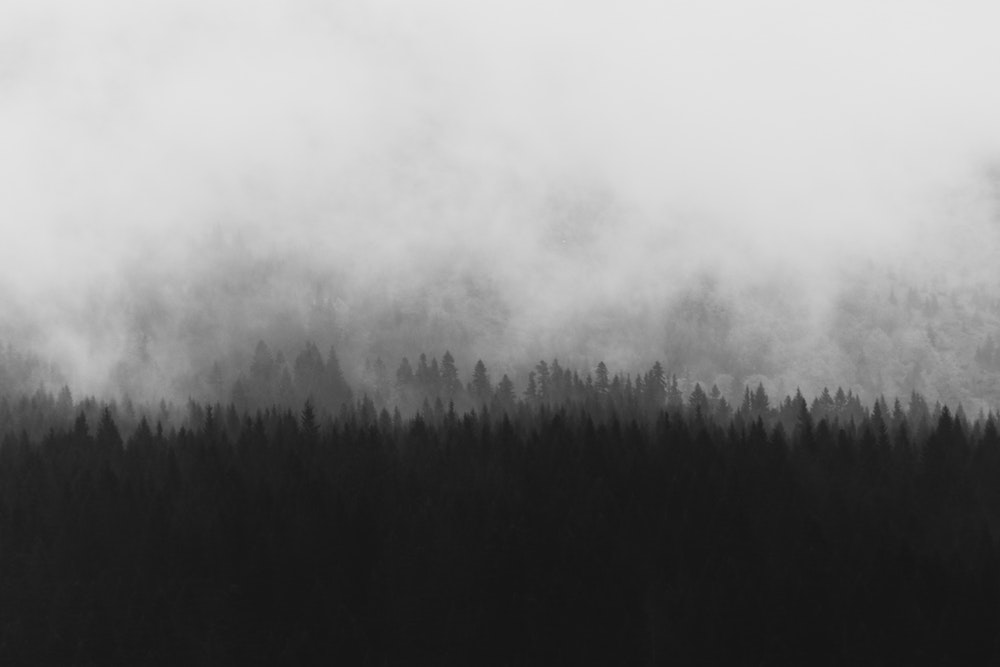
\includegraphics[width=8cm]{images/wood.jpeg}
  \caption{Originalna slika}\label{river}
\end{figure}
\columnbreak
% second column
\begin{figure}[H]
\centering
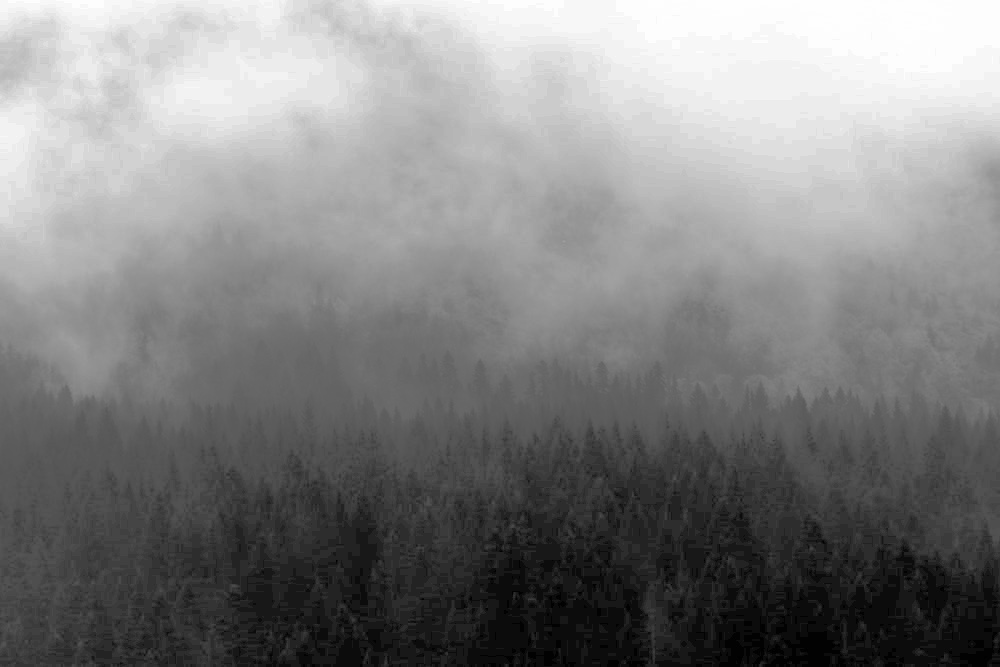
\includegraphics[width=8cm]{images/global_HE_1.jpg}
  \caption{Rezultat metode HE}\label{wood1_output}
\end{figure}
\end{multicols}

\begin{multicols}{2}
% first column
\begin{figure}[H]
\centering
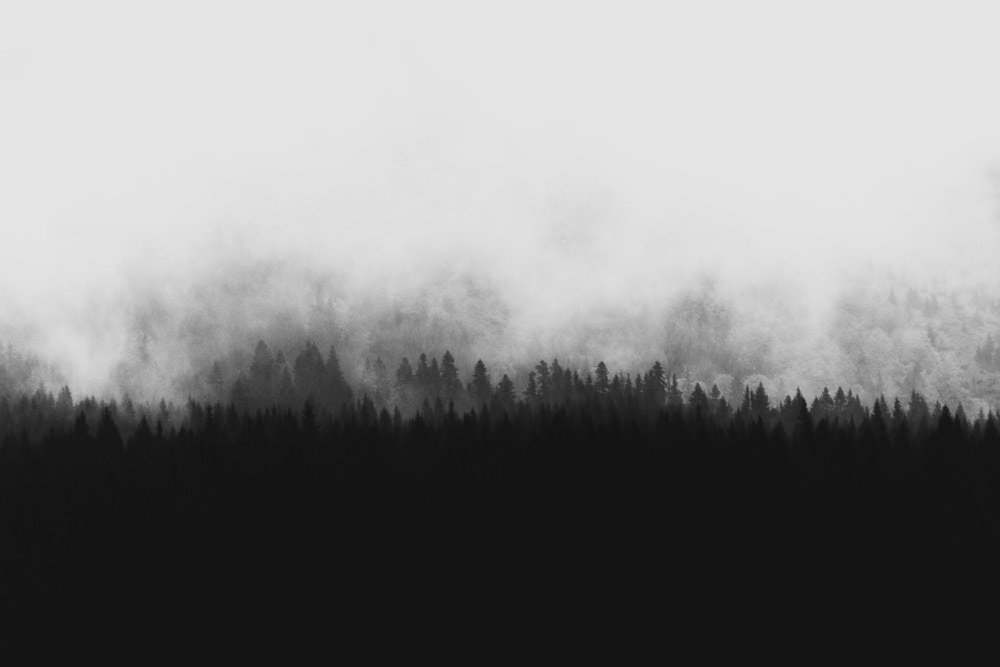
\includegraphics[width=8cm]{images/fuzzy_grayscale_1.jpg}
  \caption{Rezultat fazi metode za crno-bele slike}\label{river1}
\end{figure}
\columnbreak
% second column
\begin{figure}[H]
\centering
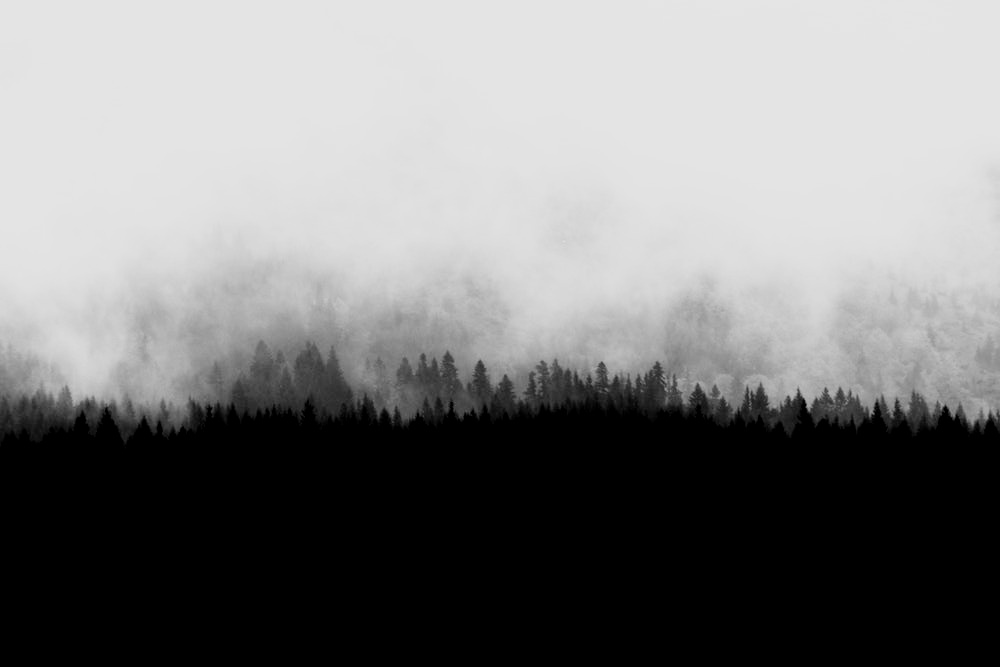
\includegraphics[width=8cm]{images/fuzzy_color_4.jpg}
  \caption{Rezultat fazi metode za slike u boji}\label{river_output1}
\end{figure}
\end{multicols}

Na osnovu dobijenih rezultata se uveravamo u to da HE metod daje rezultate vredne pa\v znje. Ponekad (Slika \ref{wood1_output}) rezultat HE metoda nije ni blizu onoga
\v sto bi uradila pandan fazi metoda. \\
Ipak, to ne zna\v ci da je rezultat lo\v siji - zavisi \v sta je posmatra\v cu potrebno od slike. U slu\v caju da je to mo\v zda ve\' ca koli\v cina informacija,
Slika \ref{wood1_output} daje najbolje rezultate. \\ 
Sude\' ci po tome koliko uspe\v sno je pobolj\v san kontrast, definitivno su pobednici fazi metode.

\newpage

\begin{multicols}{2}
% first column
\begin{figure}[H]
\centering
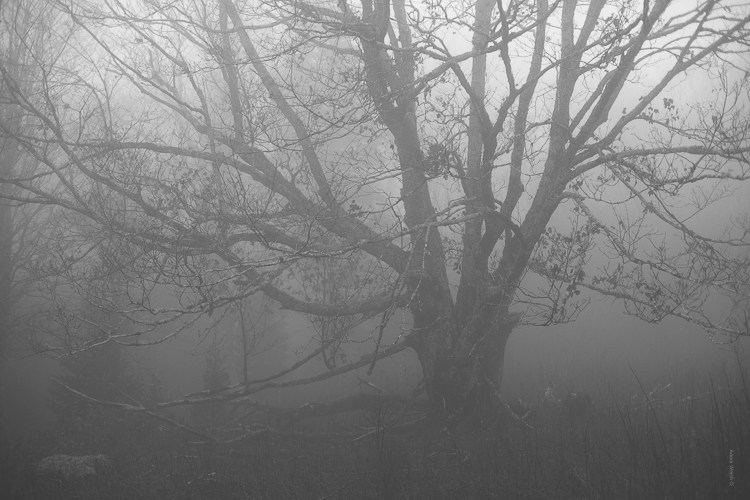
\includegraphics[width=8cm]{images/tree.jpg}
  \caption{Originalna slika}\label{river}
\end{figure}
\columnbreak
% second column
\begin{figure}[H]
\centering
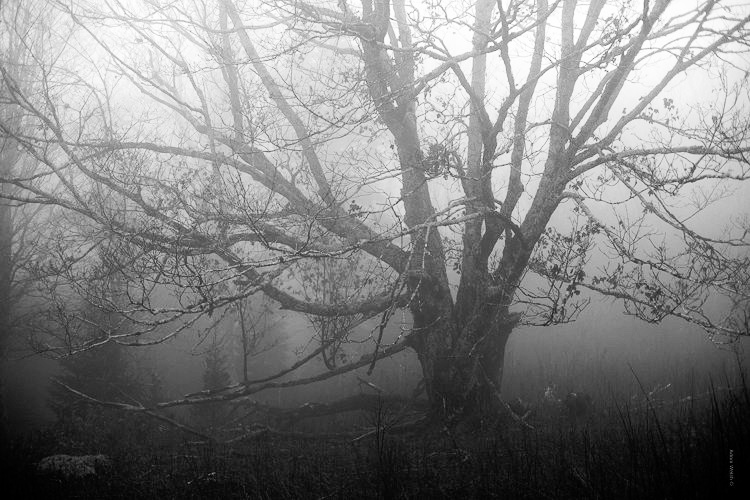
\includegraphics[width=8cm]{images/global_HE.jpg}
  \caption{Rezultat metode HE}\label{river_output2}
\end{figure}
\end{multicols}

\begin{multicols}{2}
% first column
\begin{figure}[H]
\centering
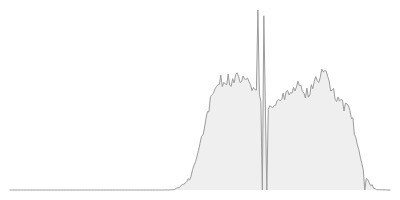
\includegraphics[width=4cm]{images/tree_hist.jpg}
  \caption{Histogram originalne slike}
\end{figure}
\columnbreak
% second column
\begin{figure}[H]
\centering
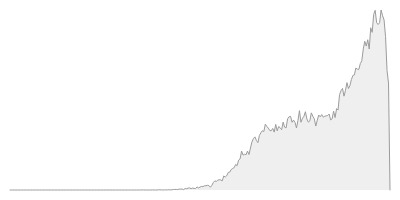
\includegraphics[width=4cm]{images/tree_HE.jpg}
  \caption{Histogram nakon HE}
\end{figure}
\end{multicols}

\begin{multicols}{2}
% first column
\begin{figure}[H]
\centering
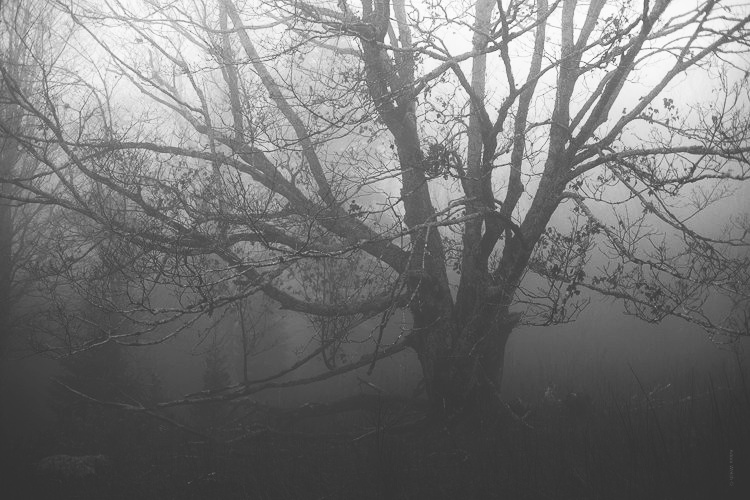
\includegraphics[width=8cm]{images/fuzzy_grayscale_0.jpg}
  \caption{Rezultat fazi metode za crno-bele slike}\label{river2}
\end{figure}
\columnbreak
% second column
\begin{figure}[H]
\centering
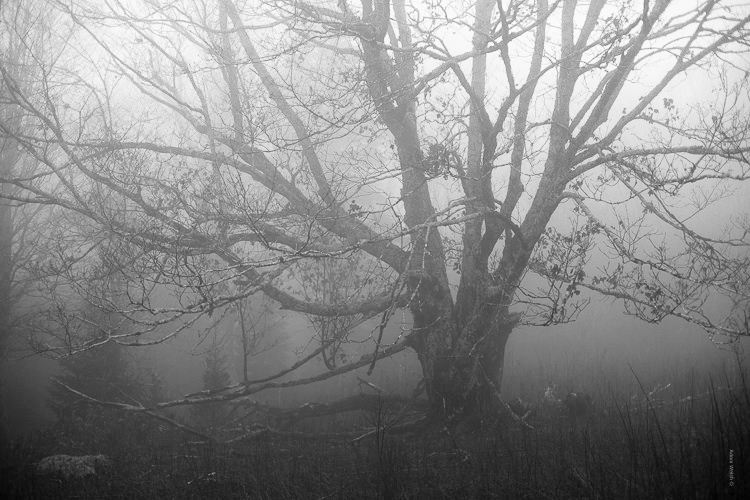
\includegraphics[width=8cm]{images/fuzzy_color_3.jpg}
  \caption{Rezultat fazi metode za slike u boji}\label{river_output3}
\end{figure}
\end{multicols}

\begin{multicols}{2}
% first column
\begin{figure}[H]
\centering
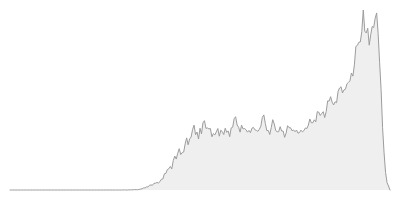
\includegraphics[width=4cm]{images/tree_gr.jpg}
  \caption{Histogram nakon fazi metode za crno-bele slike}
\end{figure}
\columnbreak
% second column
\begin{figure}[H]
\centering
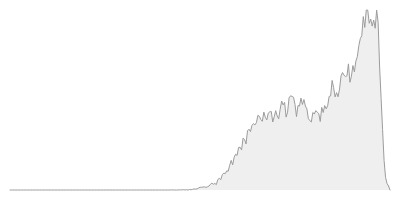
\includegraphics[width=4cm]{images/tree_color.jpg}
  \caption{Histogram nakon fazi metode za slike u boji}
\end{figure}
\end{multicols}

Kada je kontrast mera kvaliteta, fazi metode uspevaju da proizvedu ubedljivo bolje rezultate. \\
Vidno najbolje rezultate daje metoda za ulep\v savanje slika u boji. 



\newpage
\section{Zaklju\v cak}
Teorija fazi skupova i fazi logika imaju zna\v cajnu primenu u procesiranju slika. Neke od tih primena videli smo i u ovom radu - binarizacija slike, detektovanje ivica, pode\v savanje kontrasta i osvetljenosti. \\ \\
Opisana su dva algoritma, Fuzzy C-means (FCM) za binarizaciju slike i Fuzzy Edge Detection (FED) za detekciju ivica. Ovi algoritmi su pore\dj eni sa algoritmima koji ne koriste fazi logiku. Konkretno, poredili smo FCM sa k-means-om i FED sa Canny Edge Detection (CED) algoritmom. Slike dobijene FCM-om i k-means-om se skoro i ne razlikuju, dok to nije slu\v caj sa FED-om i CED-om, \v ciji su izlazi primetno druga\v ciji. U oba slu\v caja su algoritmi koji koriste fazi logiku bila br\v za.
\\
Takodje, opisana su i dva metoda za ulep\v savanje slika (slika u boji i crno-belih) koji su, u poredjenju sa tradicionalnim tehnikama zasnovanim na histogramu slike, dali mnogo bolje rezultate. \\ 
\\
Glavna prednost fazi pristupa jeste jednostavnost njihove implementacije i sposobnost da opi\v su neodredjenosti (eng. vagueness) na slikama. \\ Pored prednosti, ovi pristupi imaju i mane. Nekad to mo\v ze biti brzina izvr\v savanja, ili pak memorija. Tako\dj e, i sami rezultati se mogu dosta razlikovati od rezultata algoritama koji nisu bazirani na fazi logici, kao \v sto je to bio slu\v caj kod detekciji ivica i fazi metode za ulep\v savanje crno-belih slika.

\newpage

\begin{thebibliography}{9}
  \bibitem{} Neboj\v sa Peri\' c, "Neke primene teorije fazi skupova i fazi logike u procesiranju slika", Matemati\v cki fakultet u Beogradu, 2014.
  \bibitem{} Mario I. Chacon M, "Fuzzy binarization and segmentation of text images for opcr", Mexico New Mexico State University
  \bibitem{} Ajay Kumar Gupta, Siddharth Singh Chouhan, Manish Shrivastava, "Fuzzy based Low Contrast Image Enhancement Technique by using Pal and King Method", International Journal of Computer Applications, May 2016.
  \bibitem{} Pooja Mishra, Khom Lal Sinha, "A Highly Efficient Color Image Contrast Enhancement using Fuzzy Based Contrast", Advanced Research in Electrical and Electronic Engineering, 2014
  \bibitem{} Sankar K. Pal, Robert A. King, “Image Enhancement using Smoothing with Fuzzy Sets”, IEEE Transactions on Systems, Man and Cybernetics, July 1981.
  \bibitem{} S. N. Sivanandam, S. Sumathi, S. N. Deepa, “Introduction to Fuzzy Logic using MATLAB Springer”, Verlag Berlin Heidelberg 2007.
  \bibitem{} Hamid R. Tizhoosh, "Fuzzy Image Enhancement: An Overview", University of Magdeburg, Department for Technical Computer Science
\end{thebibliography}
\end{document}
